\documentclass{article}
\usepackage[nonatbib]{neurips_data_2021}
\usepackage[sort&compress,numbers]{natbib}
\usepackage[utf8]{inputenc}
\usepackage{booktabs}
\usepackage{hyperref}
\usepackage[capitalize]{cleveref}
\usepackage{graphicx}
\usepackage{xcolor}
\usepackage{subcaption}
\newcommand{\tbo}[1]{\textcolor{teal}{/* TBo: #1 */}}
\title{The CPD Data Set: Personnel, Use of Force, and Complaints in the Chicago Police Department}

\begin{document}


\maketitle

\begin{abstract}
The lack of accessibility to data on policing has severely limited researchers’
ability to conduct thorough quantitative analyses on police activity and
behavior, particularly with regard to predicting and explaining police
violence. In the present work, we provide a new dataset that contains
information on the personnel, activities, use of force, and complaints in the
Chicago Police Department (CPD). The raw data, obtained from the CPD via a
series of requests under the Freedom of Information Act (FOIA), consists of 35
unlinked, inconsistent, and undocumented spreadsheets. Our paper provides a
cleaned, linked, and documented version of this data that can be reproducibly
generated via open source code. We provide a detailed description of the
dataset contents, the procedures for cleaning the data, and summary statistics.
The data have a rich variety of uses, such as prediction (e.g., predicting
misconduct from officer traits, experience, and assigned units), network
analysis (e.g., detecting communities within the social network of officers
co-listed on complaints), spatiotemporal data analysis (e.g., investigating
patterns of officer shooting events), causal inference (e.g., tracking the
effects of new disciplinary practices, new training techniques, and new
oversight on complaints and use of force), and much more. Access to this
dataset will enable the machine learning community to meaningfully engage with
the problem of police violence.
\end{abstract}

\textbf{Repository: \url{https://github.com/chicago-police-violence/data}}\\
\textbf{Instructions:} run \url{make} in the repository root directory. See \url{README.md} for detailed instructions.\\
\textbf{Data Set:} may be found in the \url{final/} directory after running \url{make}.

\section{Introduction}

There has been some ML work done on individual correlates that are associated
with (and potentially predictive of) police misconduct. Scholars have looked at
the association between misconduct and an individual officer's race, gender,
years on the force, prior instances of misconduct, stages of officer career,
assigned unit. But research suggests that violence emerges not just at the
individual level but also at the population level from the interaction of
individuals in groups—think of gangs. 

 
We offer a dataset that allows ML to investigate the influence of police social
networks on police misconduct. The dataset allows ML to explore features of
police social networks that might be associated with and potentially predictive
of adverse police encounters with civilians or other misconduct. These network
correlates can include the architecture and structures of social networks in
departments and smaller subunits within a department—for example, the number of
connections each officer has, the strength of those connections, the bridge
positions that some officers have across subunits. More innovatively, ML can be
used in the way it is often used to study disease dynamics: ML can find the
patterns of behavior (clustering, outbreaks, spreading, geographic hotspots) on
a network that might be associated with violence. 

 
We show how to use complaint datasets from a police department in a major city
to investigate the influence of social networks on police misconduct and
violence. 


The original data was obtained following a series of requests covered by the
Freedom of Information Act (FOIA) to the Chicago Police Department (CPD) and
the Civilian Office of Police Accountability (COPA). The information which was
requested pertained to CPD's personnel and its activities.

\textbf{TODO:} ideally say a bit more about the history of these FOIA requests.
Apparently they were initiated by individual journalists and lawyers and were
later coordinated by the Invisible Institute which ultimately became the
central location were (almost) all the data is currently available.

\begin{table}[h]
	\begin{center}
\begin{tabular}{@{}llll@{}}
	\toprule
	request \#&received&requested&description\\
\midrule
	\texttt{P0-58155}&2017-04-17& &Officer roster\\
	\texttt{P4-41436}&2018-03-21& &Officer roster\\
		\texttt{P0-52262}&2016-12-04&2016-09-19&Unit assignment\\
		\texttt{16-1105}&2016-03-11&2016-02-10&Unit assignment\\
	\texttt{P0-46957}&2016-06-29&2016-04-22&Complaints (CPD)\\
	\texttt{18-060-425}&2018-08-28&2018-08-20&Complaints (COPA)\\
	\texttt{P0-46360}& & &Tactical Response Reports\\
\bottomrule
\end{tabular}
\caption{Summary of the FOIA requests to the CPD and COPA contained in our repository.}
\label{table:summary}
\end{center}
\end{table}

Each FOIA request is identified by a request number, \cref{table:summary} gives
an overview of all the requests made to the CPD and COPA that are present in
our repository. This information is also available in the file
\texttt{dataset.csv} in the root folder of the repository. The original
data—that is the files received after each FOIA request—are present in the
\texttt{raw/} folder of the repository, with one subfolder for each request,
identified by the request number. When available, each subfolder also contains
the formal request letter as well as the reply letter from the CPD or COPA,
which are useful in understanding what data was included in each dataset.
Some additional comments about the data:
\begin{itemize}
	\item \emph{Officer roster:} lists all officers (past or present) employed
		by the CPD along with attributes such as year of birth, age, race,
		gender, appointment date, resignation date, etc.
	\item \emph{Unit assignment:} the CPD is organized into (500 or so?) units.
		Each officer can be assigned to one or multiple units and these
		assignments can change over time. The unit assignment datasets contain
		one record for each officer and each unit they were assigned to, with
		the start date and end date of this assignment.
	\item \emph{Complaints:} formal complaints filed by citizens against police
		officers. Complaints are identified by a complaint number, and there is
		one record for each complaint and each officer listed on the complaint,
		indicating the allegation made against them, result of the
		investigation of the allegation (with possible sanction), etc.
	\item \emph{Tactical Response Reports:} these are forms that officers are
		required to file after each incident for which the officer's response
		involved use of force.
\end{itemize}

Let us already mention an inherent difficulty in making use of this data, which
will be discussed in \cref{sec:linking}: there is no number/identifier which
uniquely identifies officers across datasets. Such an identifier probably
exists internally in the CPD, but was never included in the data released to
the public. One would be tempted to believe that the \emph{badge number} (also
sometimes referred to as \emph{star number} of an officer is such an
identifier, but unfortunately, it changes over the course of an officer's
career in the CPD, and a given badge number can be reassigned to different
officers when they are no longer in use.


\subsection{Related Work}

Police records datasets

This data was originally obtained by the Invisible Institute and has been publicly available for about 3 years here \url{https://github.com/invinst/chicago-police-data}
(limitations: not well organized or reproducible, problematic/incorrect linkage, missing unit information, units are not semantically grouped)

Gang violence data



\section{The CPD Data} \label{sec:data}
The original raw data released by the CPD, 
the code to generate the cleaned data, and the source code for this document 
are available at \url{https://github.com/chicago-police-violence/data}.
The data processing code is written in Python, and the documentation is written in \LaTeX.
\texttt{Make} is used to coordinate the various processing steps and easily reproduce them.
Refer to \url{README.md} in the repository for details regarding system requirements and 
how to generate the cleaned data.

\subsection{The raw data: origin, description, and challenges}
The first raw data files in this repository were obtained by J.~Kalven, an 
independent journalist, who filed Illinois Freedom of Information Act requests with 
the Chicago Police Department regarding complaints filed against officers. 
In Kalven v.~City of Chicago \cite{kalven2014}, an Illinois appellate court issued
a general ruling that documents bearing on allegations of
police abuse are public information. Following 
the decision, the non-profit
Invisible Institute began to collaborate with Kalven 
and the University of Chicago's Mandel Legal Aid
Clinic to follow up on earlier FOIA requests and to file new ones. The data
disclosed in response to these earlier and now ongoing FOIA requests were made available
online as part of the Citizens Police Data Project \cite{cpdp}.
These data form the basis of the cleaned and linked data set provided by the present work.

\begin{table}[h]
	\begin{center}
\begin{tabular}{@{}lllll@{}}
	\toprule
	request \#&received&requested&description\\
\midrule
	\texttt{P0-58155}&2017-04-17& &Officer roster\\
	\texttt{P4-41436}&2018-03-21& &Officer roster\\
	\texttt{P0-52262}&2016-12-04&2016-09-19&Unit assignments\\
	\texttt{16-1105}&2016-03-11&2016-02-10&Unit assignments\\
	\texttt{P0-46957}&2016-06-29&2016-04-22&Complaints (CPD)\\
	\texttt{18-060-425}&2018-08-28&2018-08-20&Complaints (COPA)\\
	\texttt{P0-46360}& & &Tactical Response Reports\\
	\texttt{P0-46987}&2016-05-13&2016-04-25&Unit names\\
	\texttt{P0-61715}& &2017-07-26&Awards\\
	\texttt{P5-06887}&2019-10-11&2019-07-19&Awards\\
	&2017-09-27&2017-09-13&Salary\\
\bottomrule
\end{tabular}
\caption{Summary of the FOIA requests contained in our repository (blanks are missing entries).}
\label{table:summary}
\end{center}
\end{table}

The raw data files are contained in the \url{raw/} folder of the
repository. Each subfolder corresponds to a FOIA request, which is
generally identified by a request number. \cref{table:summary} gives
an overview of all the requests that we include in
our repository; this meta-information is also included in the \url{raw/datasets.csv}
file in the repository. The subfolders contain the data provided by the city
in response to their corresponding FOIA requests, which typically comprises multiple
Excel spreadsheets. In addition, when available, the subfolders contain formal correspondence 
regarding the request, which often provides useful contextual information in understanding the data.  

In particular, the raw data files contained in the repository
provide the following information: {\color{red} todo: year ranges for each?}
\begin{description}
	\item[Officer roster:] a list of all officers (past and present) employed
		by the CPD along with attributes such as year of birth, age, race,
		gender, appointment date, resignation date, etc.
	\item[Unit assignments:] the CPD is organized into over 200 units.
		Each officer can be assigned to one or multiple units and these
		assignments can change over time. The unit assignment datasets contain
		one record for each officer and each unit they were assigned to, with
		the start date and end date of this assignment.
	\item[Complaints:] formal complaints against police officers, filed both by citizens
                and internally within the department. Complaints are identified by a complaint number. 
                There is one record for each complaint and each officer listed on the complaint,
		indicating the allegation made against them, result of the
		investigation of the allegation (with possible sanction), etc.
	\item[Tactical Response Reports:] these are forms that officers are
		required to file after each incident for which the officer's response
		involved use of force. Each record contains... {\color{red} thibaut fill in, similar to above for complaints}
        \item[Unit names:] the (human-readable) name of each (past and present) unit in the CPD. 
                Unit names also appear occasionally where unit numbers are listed in the other data files.
        \item[Awards:] a list of all awards requested for officers in the CPD, including 
                award tracking number, reference number, award type, request date, requester name,
                etc.
        \item[Salary:] a list of officers from 2002--2017 including their salary, position, and pay grade.
\end{description}

Challenges:
- time varying attributes: badge numbers (stars), unit numbers, job titles change over time. but 
more unusual things change too -- names (e.g.~marrying), appointment dates (e.g.~when db entries are corrected)
- systematic errors: unit history backwards, 
- multiple DBs: salary comes from different DB from the rest of it. names were entered differently, etc.
- ambiguous field meanings: salary has 2 different dates for apt, etc.
- dead entries: 
- inconsistent entries across different files: officers missing from history, roster, present in salary, etc
- idiosyncratic errors: 


\subsection{Initial Cleaning}

The files initially released by the CPD as a reply to the FOIA requests are for
the most part Excel spreadsheets, with inconsistent formatting and which can
thus be difficult to process programmatically. As an example, the reader is
invited to open the file
\texttt{p046957\_-\_report\_1.1\_-\_all\_complaints\_in\_time\_frame.xls}
available in the folder \texttt{raw/P0-46957/}. As can be seen, each record in
this file is spread over two rows of the spreadsheet, with the field names
repeated at the beginning of the second row for each record.

The goal of the cleaning step is thus to produce ``reasonable'' CSV files from
the original files, with the minimum requirement that each record be presented
on a single line after this step. The code for this cleaning step is contained
in the files \texttt{datasets.py}, \texttt{parse.py} and
\texttt{parse\_p046957.py} in the \texttt{src/} folder and the entire step can
be applied by running \texttt{make parse} in the root of the repository. This
creates the folder \texttt{parsed/} containing the clean CSV files.

As can be seen by inspecting the code, the decisions made at this stage are, we
believe, uncontroversial as they only consists of:
\begin{itemize}
	\item unifying field names across datasets, so that the same type of data
		is always identified in the saw way (for example, \texttt{Appointment
		Date}, \texttt{Appt Date}, \texttt{appointment\_date} are all mapped to
		\texttt{appointment\_date}.
	\item unifying field values across datasets. For example, the gender of an
		officer is indicated as a single letter \texttt{M} or \texttt{F} in
		some datasets or as \texttt{Male}, \texttt{Female} (based on the data
		release, it does not seem that the system used by the CPD has an option
		to represent non-binary officers).
	\item parsing values into the correct data type or format. For example,
		dates are formatted differently depending on the dataset, and we map
		everything to the ISO 8601 format.
\end{itemize}

Consequently, for someone planning to use the data in the present repository,
there is virtually no reason not to start at the minimum from the output of
this cleaning step. The subsequent steps required making more difficult and
debatable decisions, so depending on the application, researchers might want to
perform them differently, but in all cases, those alternative decisions can
branch off from the output of the cleaning step.

\subsection{Linking and Merging Datasets}\label{sec:linking}

\subsubsection{Officer matching}

As already alluded to, the main challenge at this step is that there is no
identifier uniquely identifying officers across records. In other words, there
is no foolproof way to know if two different records correspond to the same
officer, \emph{even within the same dataset} (for example the same officer
could appear with slightly different attributes on two different complaint
records).

We thus need to design a matching method striking a balance between
\begin{itemize}
	\item being loose enough to avoid type II error (false negatives). If the
		same officer appears with slightly different attributes across two
		records, we do not want our matching method to believe it is two
		different officers.
	\item being strict enough to avoid type I error (false positives). We do
		not want to merge two different officers into a single identity.
\end{itemize}

The difficulty in achieving this balance is that perhaps surprisingly
\emph{none of the attributes of a given police officer are guaranteed to be
stable over time}. Most notably, officers' names change over time, for example
to fix data entry errors or in case of legal name changes. However, we observed
two attributes, present in almost all original datasets and which seem
remarkably stable over the time: \emph{appointment date} and \emph{birthyear}.
These two attributes thus proved very valuable to disambiguate officers with
identical names.

In order to match officers across two datasets, we developed an \emph{iterative
pairwise matching procedure} that makes iterative passes over the datasets.
During each pass, a subset of the officer attributes present in both datasets
is selected as the matching criterion, and a pair of officers (one from each
dataset) is identified as a \emph{match} if (i) their attributes from the
chosen subset match, and (ii) if they are the only two officers matching on
these attributes. Once a pair is identified as a match, it is put aside, and
the next pass is performed on the remaining unmatched officers. After all the
passes are done the leftover officers are declared as different officers. By
constructing a hash table mapping a subset of attributes to the list of
officers sharing these attributes, each pass can be performed in linear time,
so the overall running time of the procedure is $O\big(P(N_1+N_2)\big)$ where
$P$ is the number of passes and $N_1, N_2$ are the number of officers in each
dataset.

To fully specify the matching procedure we thus need to specify which subset of
attributes is chosen as the matching criterion at each pass. For this, we go
from the stricter to the looser criterion: for the first pass, we choose
a subset \emph{all} the attributes which are present in two datasets, and then
start removing attributes one by one. For example, one can remove the
\emph{last name} attribute for the second pass to match a pair of officers
whose last names are different but match on all the remaining attributes, thus
identifying an officer whose last name changed between the releases of the two
datasets. The advantage of going from stricter to looser is two fold:
\begin{itemize}
	\item starting from the strictest set of attributes identifies the
		\emph{unambiguously matching pairs}, that is, the ones which are
		a clear match and which, thankfully, constitute the vast majority of
		officers (typically around 80-90\% of officers are matched during the
		first pass \textbf{TODO check}). Since the next passes will only be
		performed on the remaining unmatched officers, this removes a lot of
		potential ambiguities which could occur once the set of attributes is
		reduced.
	\item since the vast majority of officers is matched during the first pass,
		it becomes feasible during the subsequent passes to visually inspect all
		the matched pairs and assess whether the chosen set of attributes was
		too strict or too lose (\textbf{TODO:} explain how to activate
		debugging information in the code).
\end{itemize}

We note that there is still some amount of subjective judgment involved,
following a visual inspection of the second and subsequent passes, to decide
which sets attributes are ``acceptable'' (that is, for which the probability of
two persons sharing these attributes in a population of the size of the CPD is
extremely small). This is also how we decide that sufficiently many passes have
been performed: when it would seem likely to introduce a type I error by
matching any of the remaining officers. As a general rule of thumb we erred on
the side of favoring type II errors over type I errors. That is, we only
matched officers when it would seem extremely unlikely that they correspond to
two different individuals).

\textbf{TODO:} table of officer attributes in each dataset

\textbf{TODO:} explain the few subtleties where we don't use equality to match
attributes (for example when matching age and birthyear, where the age only
lets us identify the birthyear with an accuracy of 1 year). Or with stars,
where we test whether a star number is contained in the subset of known stars
for this officer.

With this procedure at hand we can thus link officers across datasets starting
from the most similar datasets first (for which we expect to have the least
amount of ambiguity). That is we first link \texttt{P0-58155} to
\texttt{P4-41436}, then \texttt{P0-52262} to \texttt{16-1105} and then the
remaining datasets \textbf{expand}

\textbf{TODO} give in appendix table summarizing which subset of attributes are
used at each linking operation 

\subsubsection{Roster consolidation}

A byproduct of matching officers across datasets is that for each officer, we
now have as many “profiles” as the number of datasets in which they appear,
where by \emph{profile} we mean a collection of attributes. Note that each
profile can contain a different subset of attributes (since not all attributes
are present in each dataset) and that a given attribute might take a different
value in different profiles of the same officer (since the iterative matching
procedure is not restricted to performing strict matching).

We are thus faced with the task of “consolidating” the different profiles of
a given officer into a single profile. Of course, if an attribute is present in
a single profile, and absent from the others, this is the value we keep in the
consolidated profile. But if an attribute appears with different values across
different profiles, we choose the value coming from the profile corresponding
to the \emph{most recent data release}.

\subsubsection{Unit assignment history} TODO.


\subsection{Unit identification and binning}


% !TEX root = ../main.tex

\section{Exploratory Analysis and Examples} \label{sec:analysis}

In this section, we provide examples and use-cases on the dataset. Code to
reproduce our examples is available online, in the \texttt{examples} folder.

\subsection{Visualizations}

\paragraph{Roster.}
%The file \texttt{roster.csv} contains information about $N=35{,}430$ CPD
%officers. For each officer --- identified by a Unique Identifier (``uid''),
%\texttt{roster.csv} provides, among other covariates, the officer's name,
%gender, race, birthyear, appointment and resignation dates. It is
%straightforward  to use the data to generate summary statistics, e.g., using
%appointment and resignation dates to understand the number of appointments,
%retirements as well as active officers over the years of  (\Cref{fig:history}).
%We report in \Cref{tab:stats} some 


\begin{figure}[t!] 
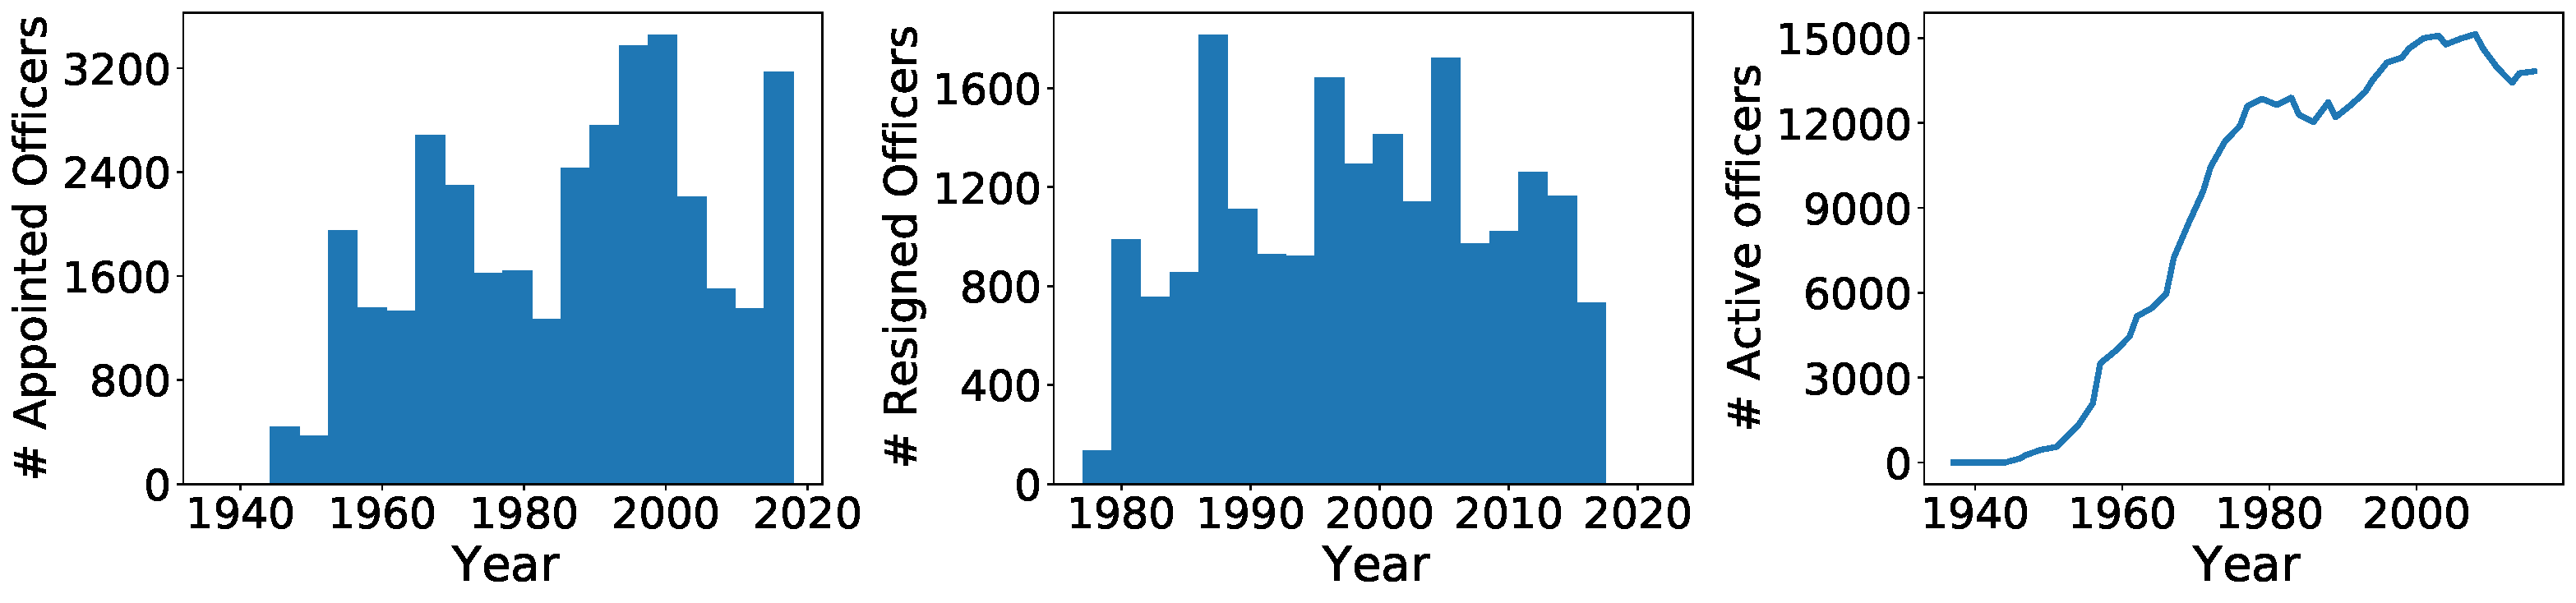
\includegraphics[width=\textwidth]{figs/history} 
\caption{Appointments (left), resignations (center), and the number of active
officers (right) appearing in the CPD roster database from the years 1940 to 2019.}
\label{fig:history}
\end{figure}

\begin{table}[t!]
\caption{Counts of officers (first row) and active officers (resignation date not before 2019-01-01, second row). 
Note that ``race'' and ``gender'' are per the CPD's coarse categorizations.} \label{tab:stats}
\begin{tabular}{l|c|c|c|c|c|c|c|c|c|}
\cline{2-3} \cline{5-10}
                                               & \multicolumn{2}{c|}{\textbf{Gender}} & \multicolumn{1}{l|}{} & \multicolumn{6}{c|}{\textbf{CPD Race Category}}                                                                                                                                                   \\ \cline{2-3} \cline{5-10} 
                                               & {\textbf{M}}   & {\textbf{F}}   &                       & {\textbf{White}} & {\textbf{Black}} & \multicolumn{1}{l|}{{\textbf{Hisp.}}} & {\textbf{Asian/P.I.}} & \multicolumn{1}{l|}{{\textbf{Indig.}}} & {\textbf{Bl. Hisp.}} \\ \cline{1-3} \cline{5-10} 
\multicolumn{1}{|c|}{\textbf{All}}    & 28316                 & 7122                  &                       & 21047                   & 8599                    & 4811                                         & 582                     & 67                                              & 9                           \\ \cline{1-3} \cline{5-10} 
\multicolumn{1}{|c|}{\textbf{Active}} & 11118                 & 4452                  &                       & 7241                    & 3895                    & 3596                                         & 467                     & 40                                              & 9                           \\ \cline{1-3} \cline{5-10} 
\end{tabular} 
\end{table}

\begin{figure}[h] 
	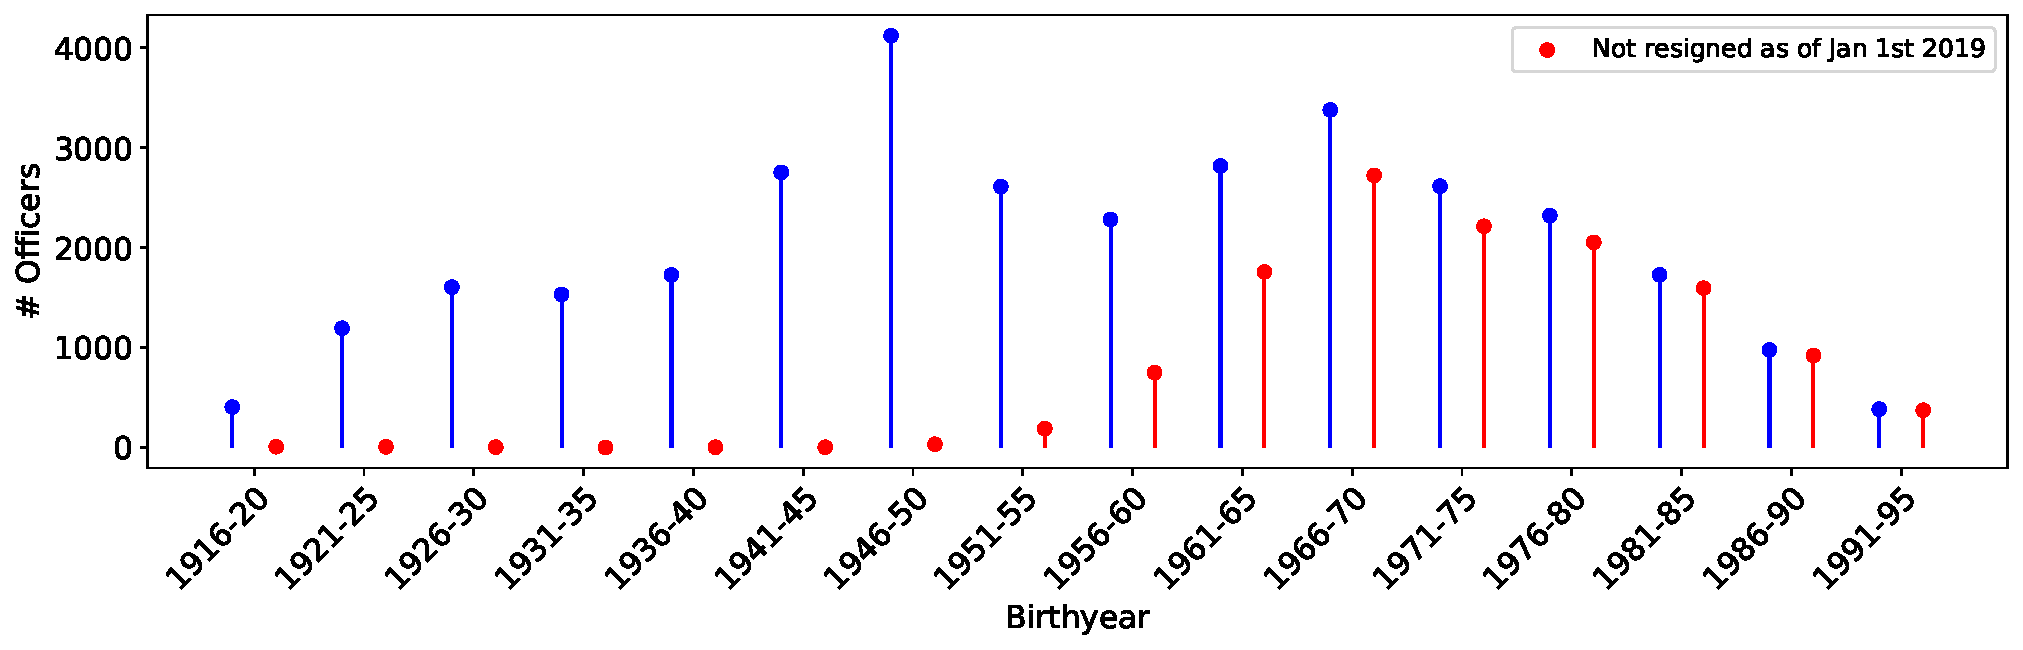
\includegraphics[width=\textwidth]{figs/history_by} 
	\caption{Historical data from the CPD. Birthyears for officers in the CPD dataset: blue dots count all officers, while red count only officers who are ``active'' as of January 1st, 2019.} \label{fig:history_by}
\end{figure}

We use the file \texttt{roster.csv} to obtain basic statistics about officers in the CPD dataset. The data contains informations about officers whose appointment dates back to 1936, all the way to 2018 (see \Cref{fig:history}). An important remark to be made is that the data becomes sparser, and less reliable in earlier years. For example, we report in the right subplot of \Cref{fig:history} the number of active officers (vertical axis) as a function of time (horizontal axis): we notice that this number increases sharply between 1940 and 1980. This should be interpreted as a consequence of the lack of data availability for those early years. We also report summary statistics on gender and the CPD race category in \Cref{tab:stats}, and information about officers' birthyears in \Cref{fig:history_by}.

\paragraph{Units.} 
\begin{figure}[h] 
	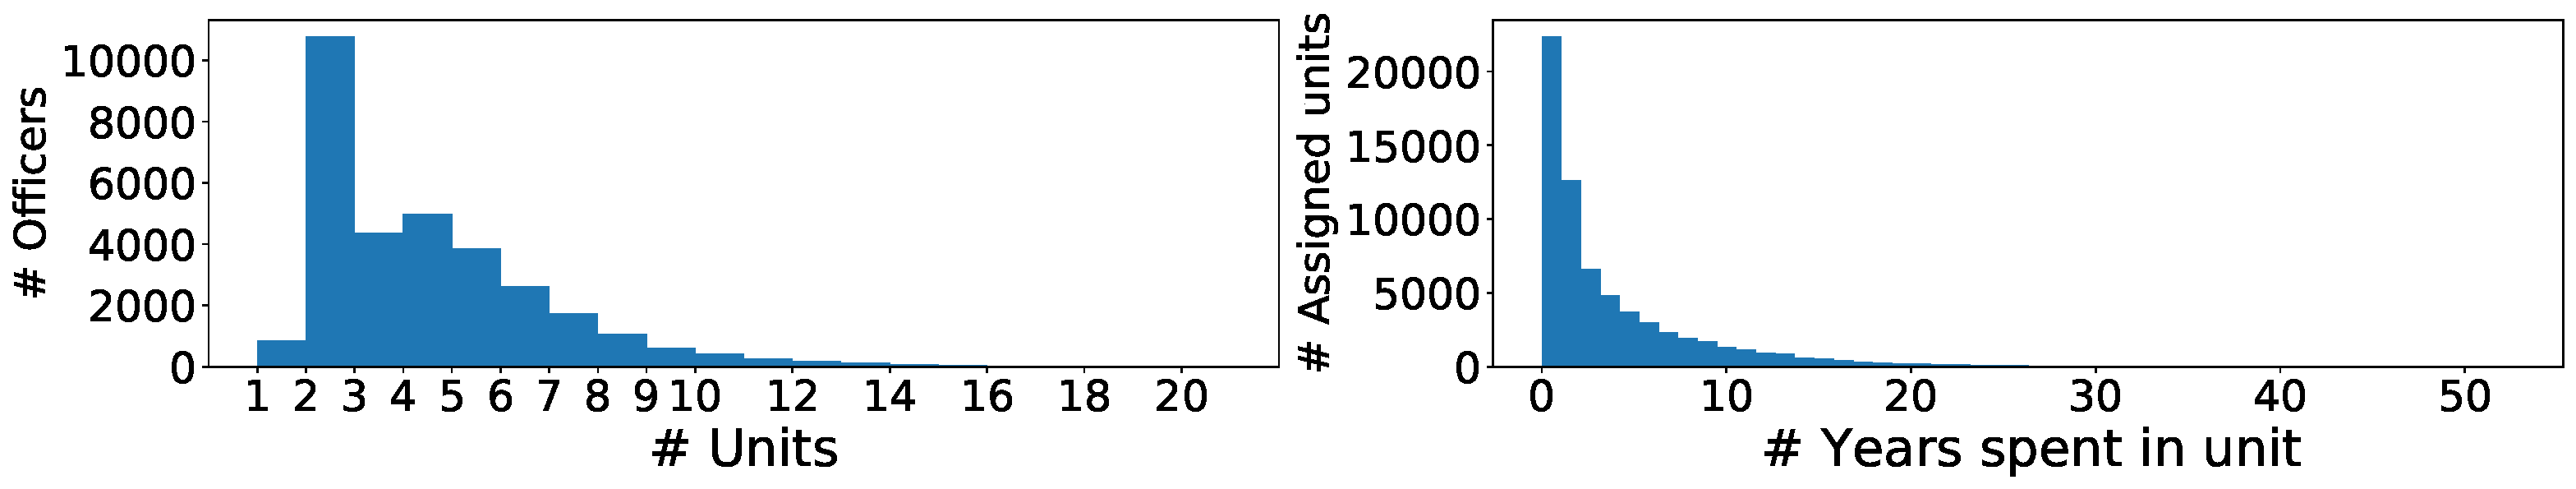
\includegraphics[width=\textwidth]{figs/units_officers} 
	\caption{Units assignments. Left: number of units assignments for officers in the CPD over the course of their career. Right: histogram for the number of years spent in each unit for ``completed'' units assignments only --- that is, assignments that had terminated at the time of data-collection.} \label{fig:units}
\end{figure}


We report summary statistics about the number of units an officer is assigned to, and the duration of such appointments in \Cref{fig:units}. The modal number of units appointments is 2: officers typically first joins the acadamy (unit 44), for one or two years, before moving on to a different, often terminal, unit. 
 
\paragraph{Complaints.} 
\begin{figure}[h] 
	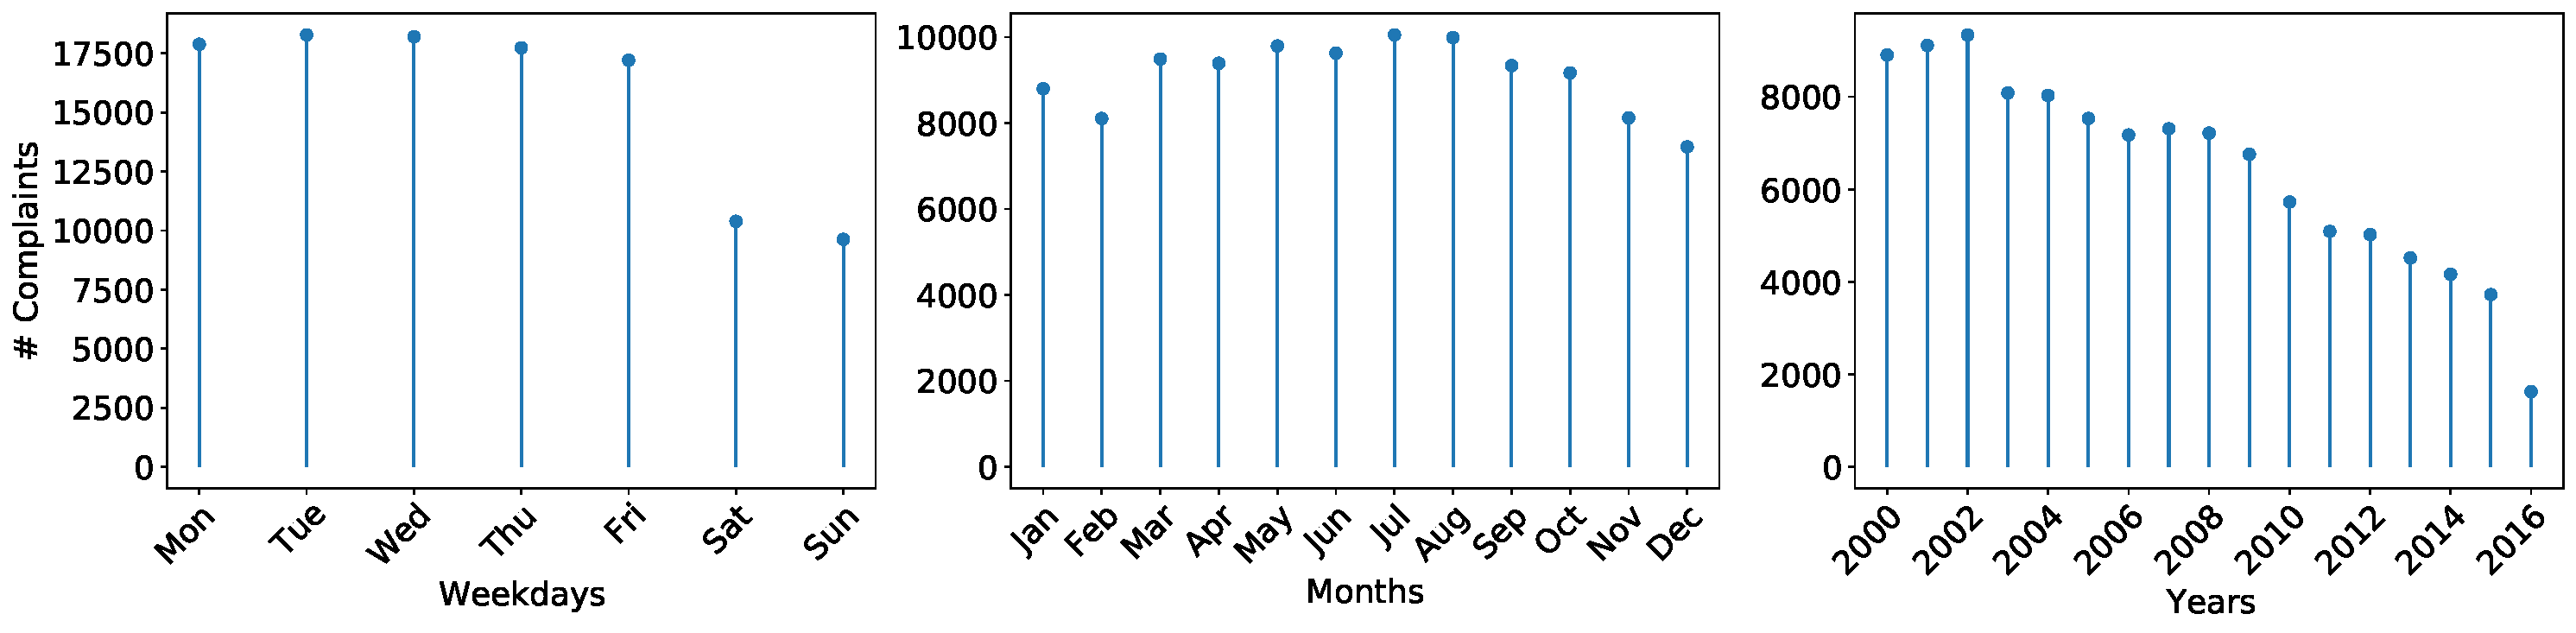
\includegraphics[width=\textwidth]{figs/complaints_times} 
	\caption{Temporal data for complaints.} \label{fig:complaints_times}
\end{figure}
\begin{figure}[h] 
	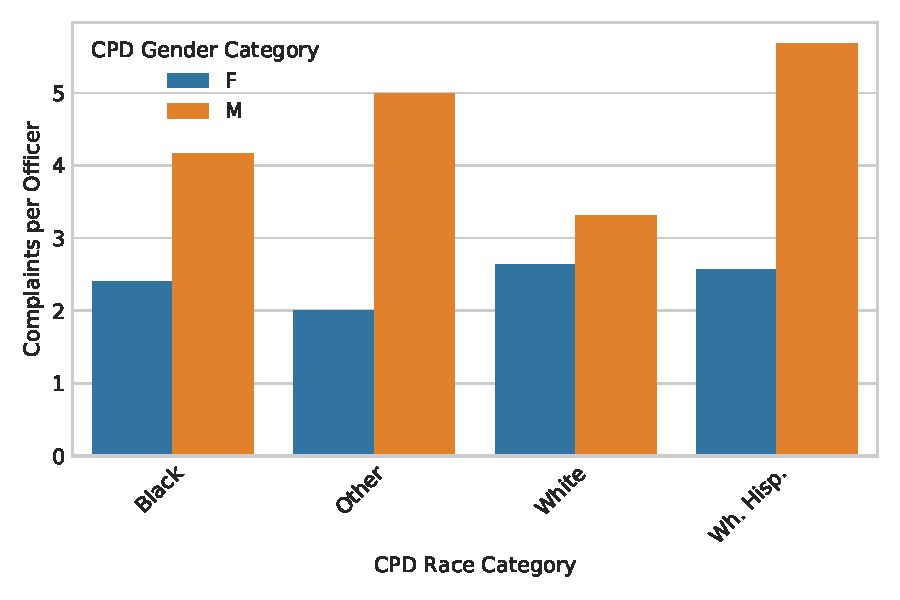
\includegraphics[width=\textwidth]{figs/complaints} 
	\caption{Temporal data for complaints.} \label{fig:complaints}
\end{figure}

We report in \Cref{fig:complaints} temporal information about complaints filed against the CPD. Interestingly, fewer complaints get filed during the weekends (although, the number of TRRs is higher then --- see \Cref{fig:trrs_times}). Moreover, complaints tend to be higher in the warmer months. Last, we notice that the number of complaints filed kept reducing over the years --- potentially as a consequence of the perception of ineffectiveness of such complaints.

\paragraph{Tactical Response Reports.}

\begin{figure}[h] 
	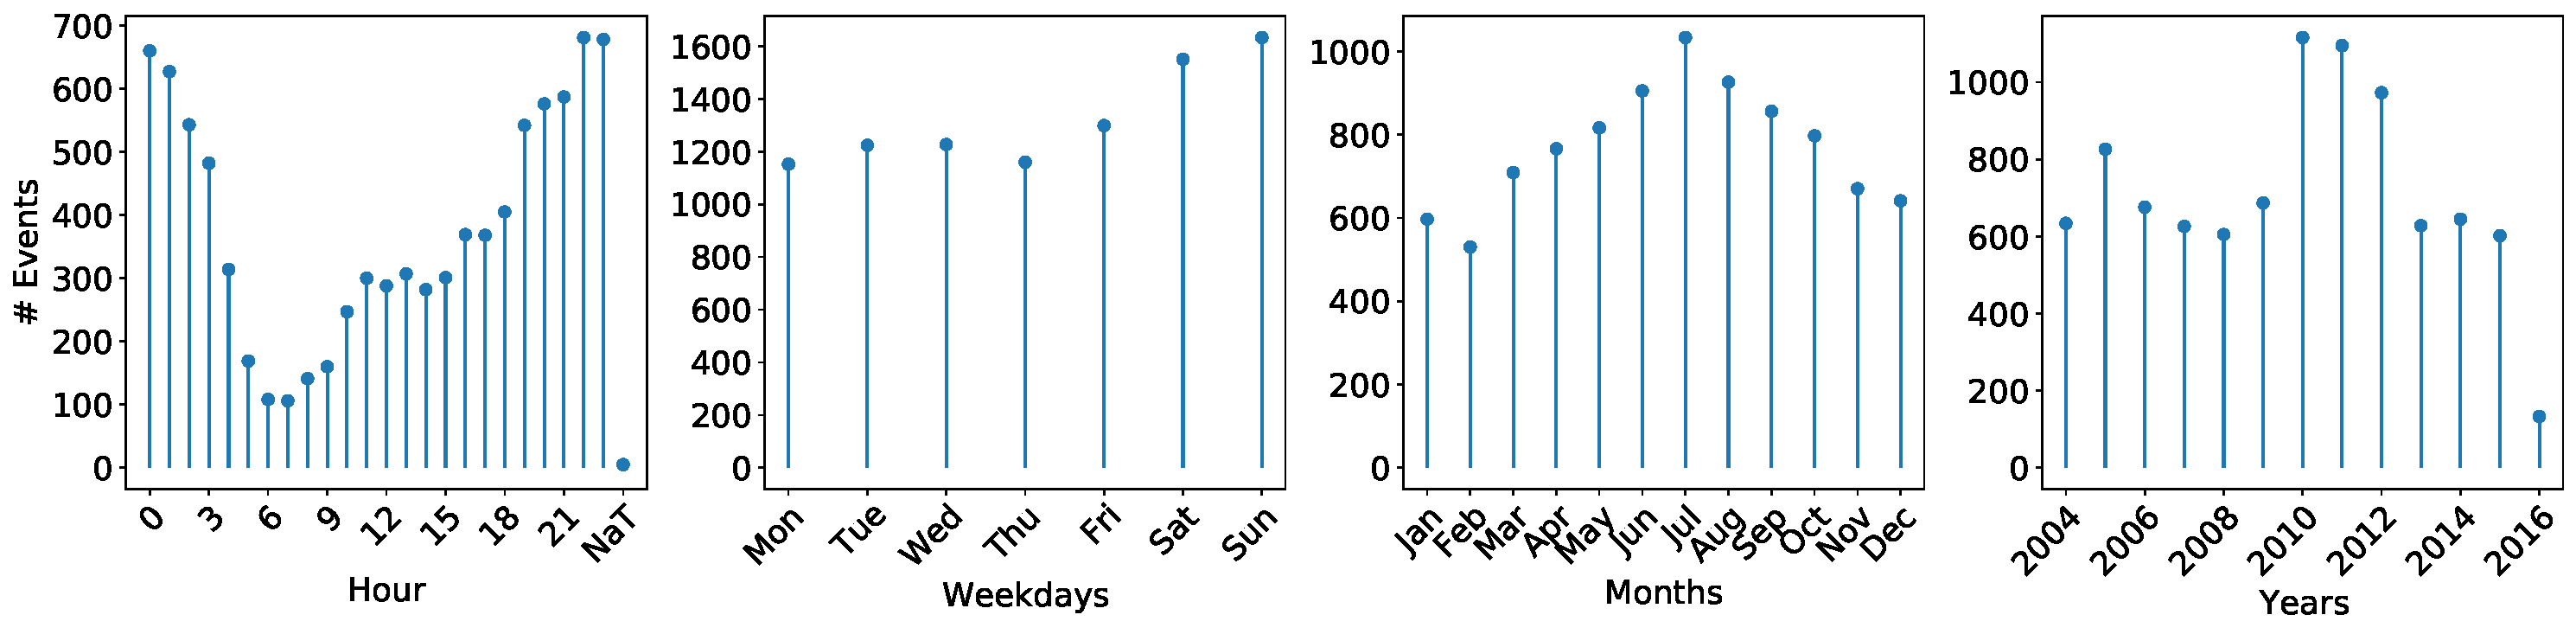
\includegraphics[width=\textwidth]{figs/trrs_times} 
	\caption{Temporal data for TRRs. Left: time during the day; mid-left: time during the week; mid-right: month; right: year.} \label{fig:trrs_times}
\end{figure}

\begin{figure}[h] 
	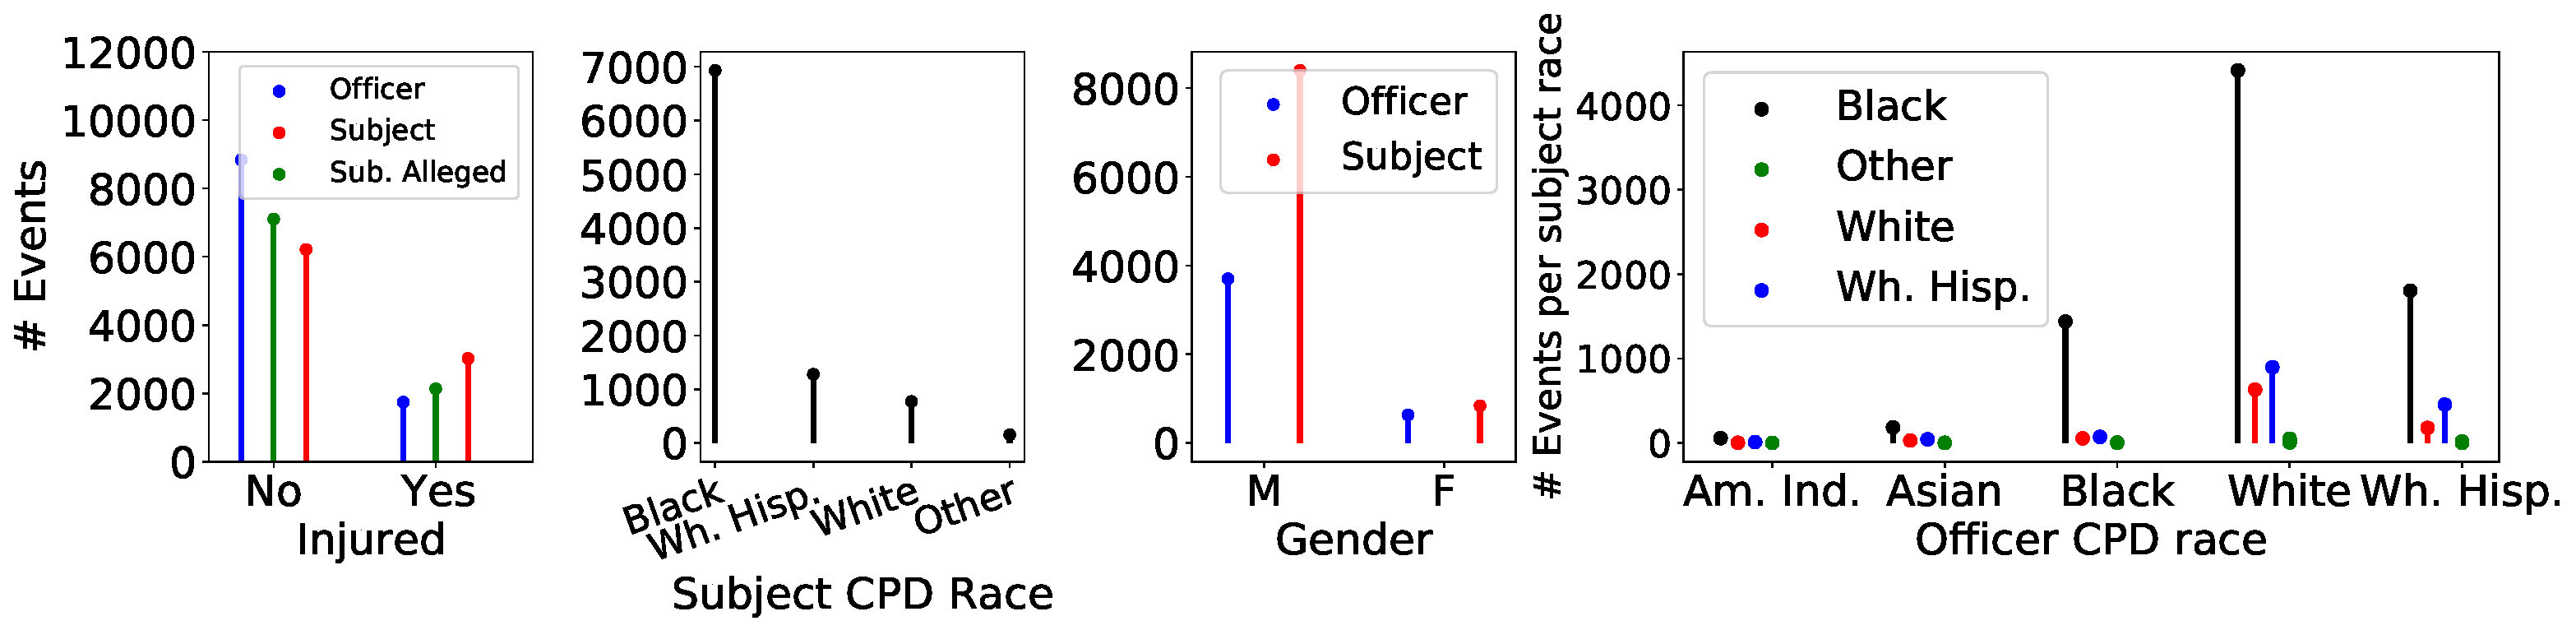
\includegraphics[width=\textwidth]{figs/trr_stats} 
	\caption{Additional statistics for TRRs.} \label{fig:trrs_stats1}
\end{figure}

%\begin{figure}[h] 
%	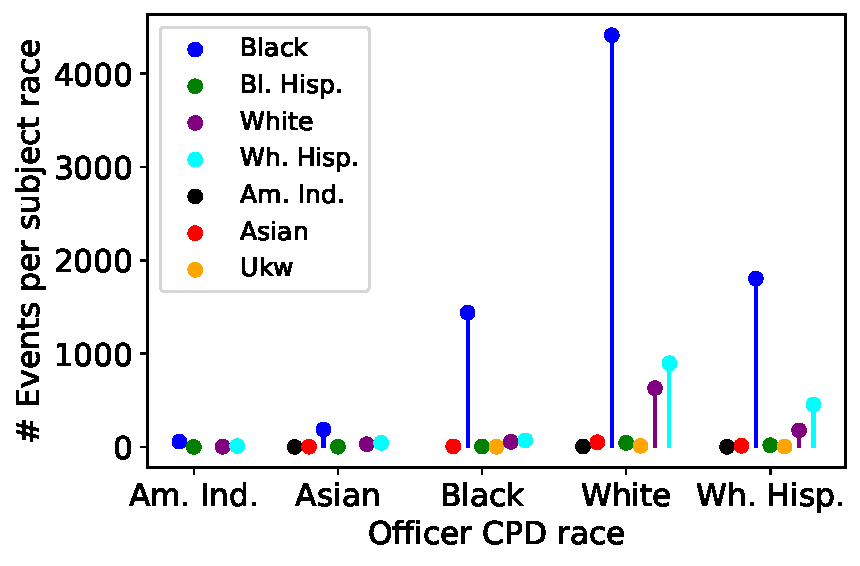
\includegraphics[width=\textwidth]{figs/trr_stats_race_race} 
%	\caption{Temporal data for TRRs.} \label{fig:trrs_stats2}
%\end{figure}

We also report temporal information about the TRRs in \Cref{fig:trrs_times}. TRRs tend to be filed more frequently at night, in the weekends, and during warmer months. Moreover, 2010, 2011 and 2012 are the years in which the highest number of TRRs have been filed. We also report in \Cref{fig:trrs_stats1} additional information about TRRs: in most cases, neither the officers nor the subjects involved get injured, although civilians get injured at a much higher rate (left subplot), and officers tend to fire first. 
\paragraph{Salary.} todo

\begin{figure}[h] 
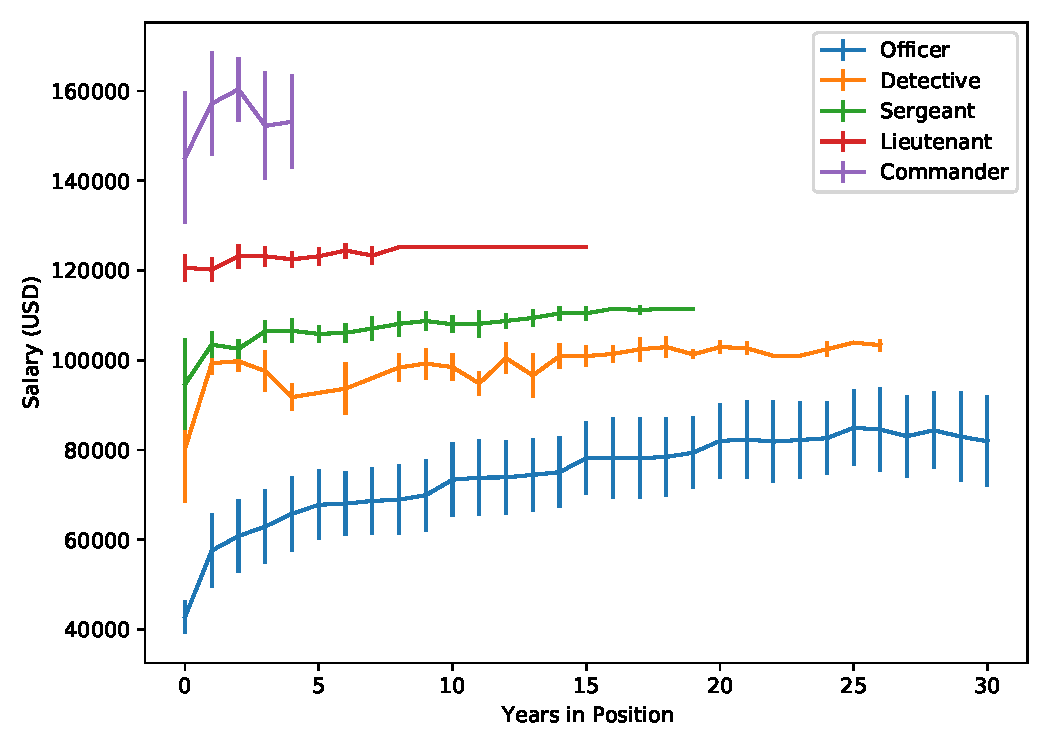
\includegraphics[width=\textwidth]{figs/salary} 
\caption{Historical data from the CPD. Salary versus experience in each
position, years x axis, salary (USD) y axis, for a few of the most common
positions. Lines are means, bars indicate 1 std dev above and below.} \label{fig:salary}
\end{figure}

\begin{figure}[h] 
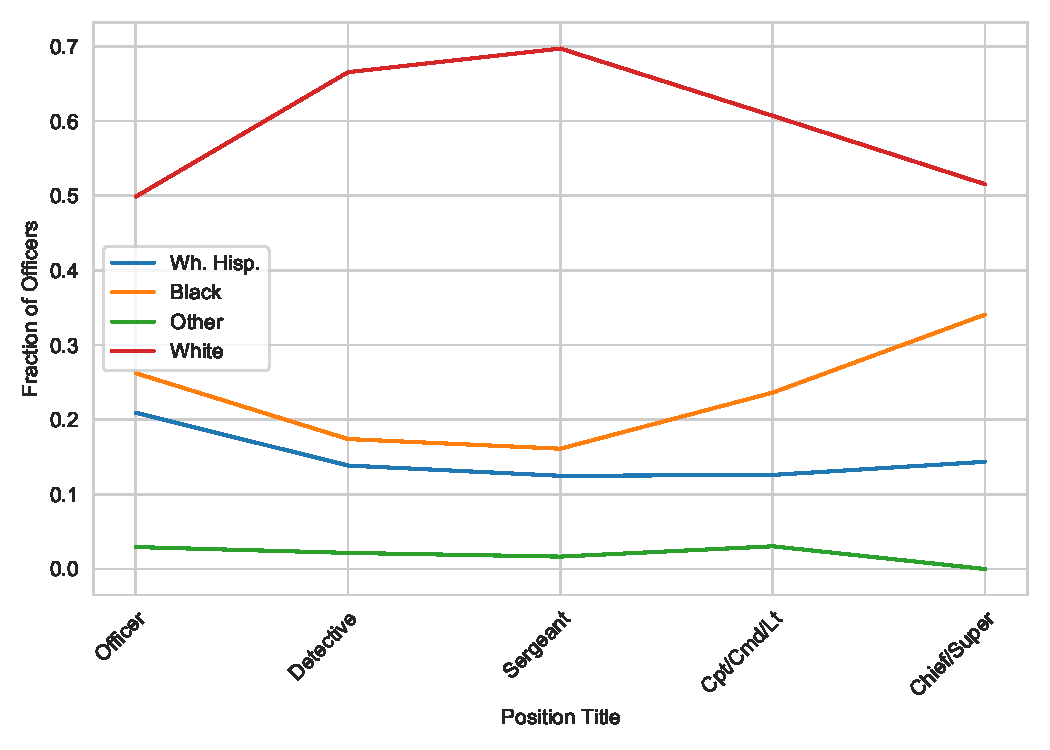
\includegraphics[width=\textwidth]{figs/position_race} 
\caption{Historical data from the CPD. Fraction of officers in representative positions 
per race category.} \label{fig:salary}
\end{figure}

\begin{figure}[h] 
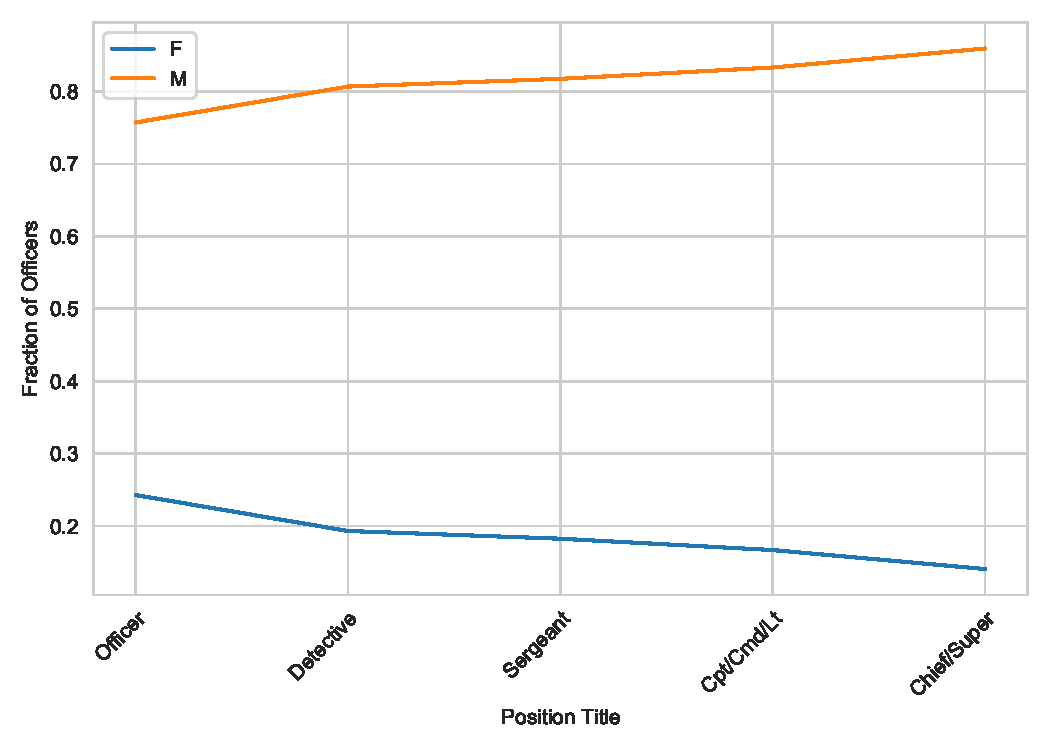
\includegraphics[width=\textwidth]{figs/position_gender} 
\caption{Historical data from the CPD. Fraction of officers in representative positions 
per gender category.} \label{fig:salary}
\end{figure}

\paragraph{Awards.}

\begin{figure}[h] 
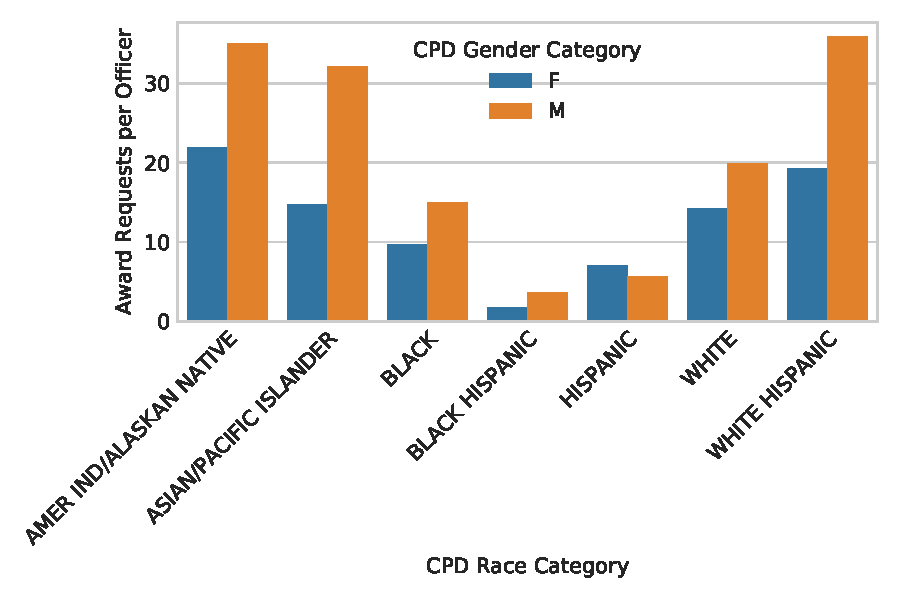
\includegraphics[width=\textwidth]{figs/awards} 
\caption{Historical data from the CPD. Awards per officer vs race for the two cpd gender categories.} \label{fig:awards}
\end{figure}




% !TEX root = ../main.tex

\subsection{Building an officers' network}

Among several tasks, we can use the CPD dataset to perform network analysis. \textcolor{red}{Should cite policing papers who do network analysis?}. For example, we can use the \texttt{complaints\_officers.csv} data to construct an undirected graph $\mathcal{G} = \{\mathcal{V}, \mathcal{E}\}$, in which $\mathcal{V}$ is the set of nodes --- officers appearing in at least one complaint, and $\mathcal{E}$ the set of edges --- where an edge is present whenever two officers appeared on the same complaint. Moreover, we can link the complaints to the \texttt{tactical\_response\_reports.csv} file, to consider also the subgraph of officers who were also listed in a TRR. We report summary for the corresponding graphs in \Cref{tab:stats_graphs}. Here, we consider any complaint available to form an edge, but we only consider TRRs filed after January 1st 2004, and before December 1st 2015.

\begin{table}[h]
\begin{tabular}{c|c|c|c|c|c|c|c|}
\cline{2-8}
                                                & $|\mathcal{G}|$ & $|\mathcal{E}|$ & \textit{Avg. degree} & \textit{Triangles} & \textit{Max clique} & \textit{LCC} & \textit{\# Is. nodes} \\ \hline
\multicolumn{1}{|c|}{\textit{\textbf{All}}}     & $14{,}372$      & $106{,}701$     & $14.85$              & $361{,}878$        & $64$                & $13{,}950$   & $0$                   \\ \hline
\multicolumn{1}{|c|}{\textit{\textbf{In TRRs}}} & $4{,}105$       & $22{,}064$      & $10.75$              & $44{,}786$         & $28$                & $3{,}822$    & $225$                 \\ \hline
\end{tabular} \label{tab:stats_graphs}
\caption{Summary statistics for the complaints network graph, and the subgraph of officers in TRRs. Here LCC is the largest connected components, and Is. nodes is the number of isolated nodes.}
\end{table}

\begin{figure}[t!] 
	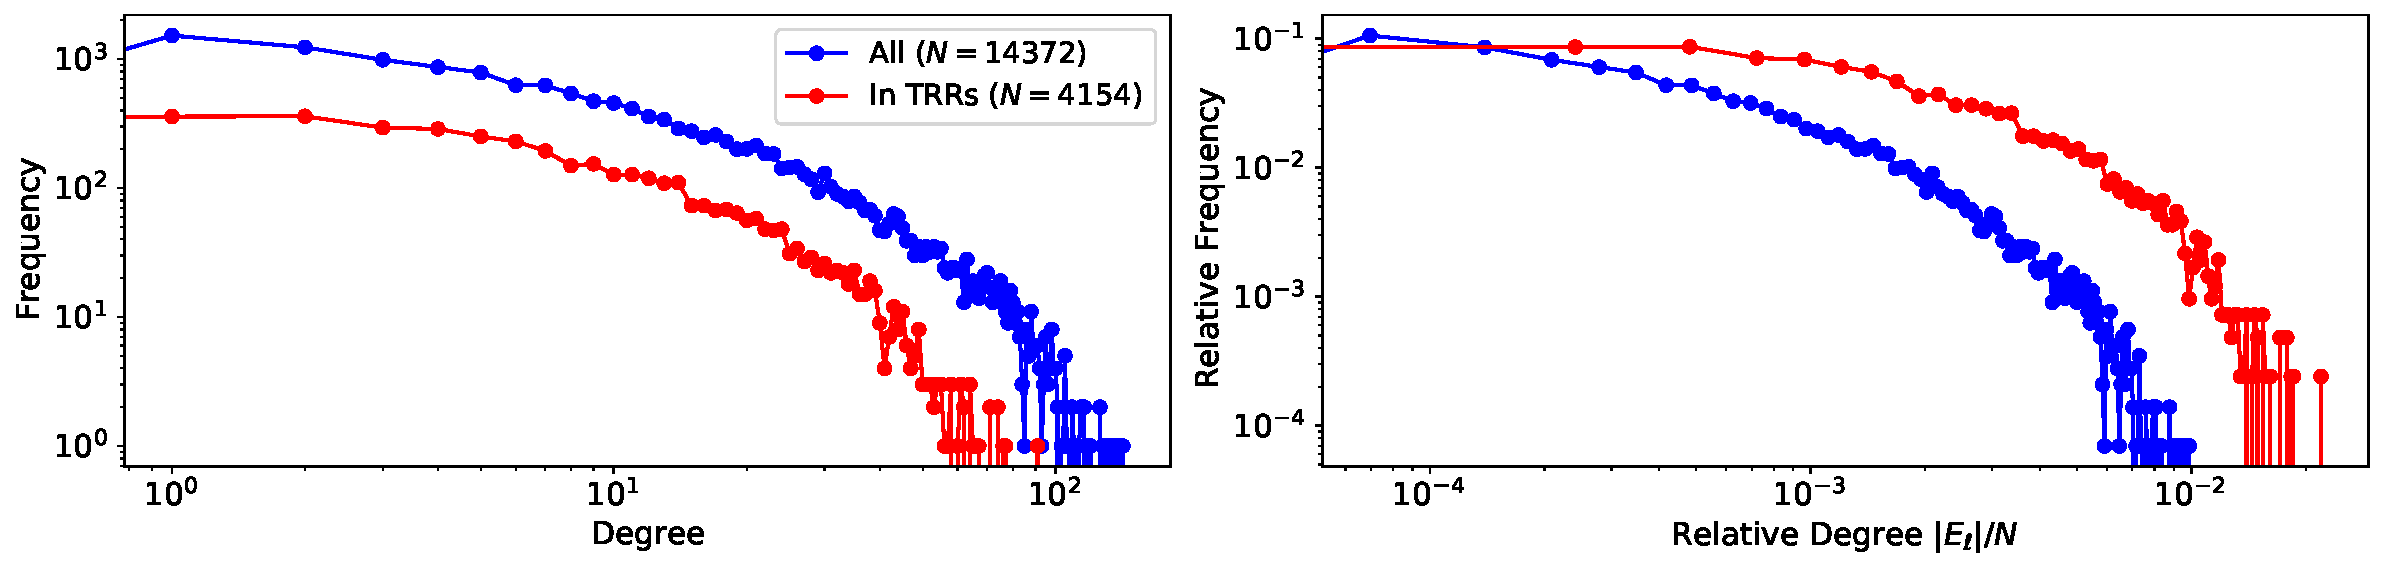
\includegraphics[width=\textwidth]{figs/degree_distribution} 
	\caption{Degree distribution for the complaints network.}
\label{fig:degree_distribution}
\end{figure}

\begin{figure}[t!] 
	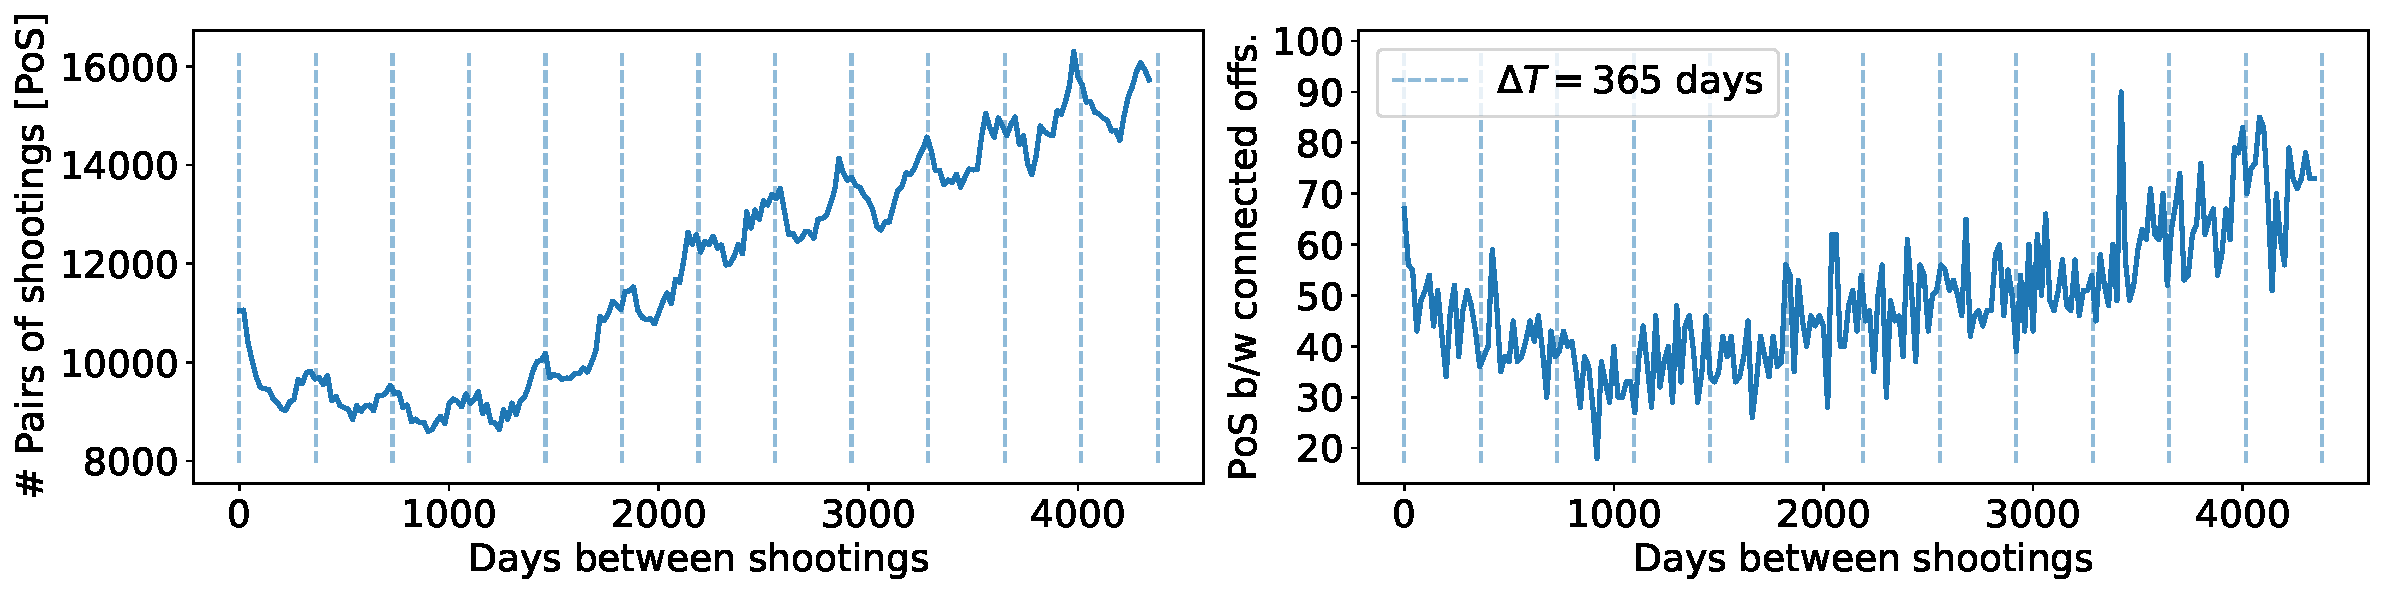
\includegraphics[width=\textwidth]{figs/intrashooting_times} 
	\caption{Intrashooting times between pairs of shootings.}
\label{fig:intrashooting_time}
\end{figure}


% !TEX root = ../main.tex
\section{Discussion} \label{sec:discussion}

\subsection{Intended Uses}
Uses for this dataset are varied and rich. For example, researchers could
use the data in a wide variety of predictive tasks, such as
predicting officer misconduct, resignation, and shooting as a function
of their underlying demographic data or complaints filed against them. Past work has engaged
in this type of analysis on both the raw data underlying the present
work, as well as confidential internal police department data \cite{Helsby18,Rozema19}.
This dataset can also be used to study social networks (both in the context of policing and more generally). 
In particular, we can use data in \texttt{complaints\_officers.csv} to construct an
undirected graph $\mathcal{G} = \{\mathcal{V}, \mathcal{E}\}$ in which
$\mathcal{V}$ is the set of nodes---officers appearing in at least one
complaint, and $\mathcal{E}$ the set of edges---where an edge is present
whenever two officers appear on the same complaint. Moreover, we can link the
complaints to the \texttt{tactical\_response\_reports.csv} file to consider
also the subgraph of officers who filed a TRR. We report summary statistics
for the corresponding graphs in \Cref{tab:stats_graphs}, with additional related visualizations
in \cref{sec:additional_figs}.
These networks are of interest in and of
themselves, but can also be used to investigate the dynamic patterns of officer
wrongdoing along such police networks \cite{Roithmayr16}. Existing research has used the complaint
data to identify such patterns and to investigate whether pairs of officers
connected on a network are more likely to have been accused of misconduct \cite{Ouellet19}.
Finally, this dataset could be used to track the effects of new disciplinary
practices, new training techniques, and new oversight on complaints and use of
force. A working paper explores, for example, whether civilians filed fewer
complaints about officers' force in the wake of the Department of Justice
investigation of the Chicago Police Department \cite{Travers20}. 


\begin{table}[t!]
\caption{Summary statistics for the complaints network graph, and the subgraph
of officers in TRRs. All complaints and TRRs filed between 
2004-01-01 and 2015-12-01 are considered in the network construction.
Here LCC is the largest connected component, and Is.~nodes is 
the number of isolated nodes. 
}\label{tab:network}
\begin{tabular}{c|c|c|c|c|c|c|c|}
\cline{2-8}
                                                & $|\mathcal{G}|$ & $|\mathcal{E}|$ & \textit{Avg. degree} & \textit{Triangles} & \textit{Max clique} & \textit{LCC} & \textit{\# Is. nodes} \\ \hline
\multicolumn{1}{|c|}{\textit{\textbf{All}}}     & $14{,}372$      & $106{,}701$     & $14.85$              & $361{,}878$        & $64$                & $13{,}950$   & $0$                   \\ \hline
\multicolumn{1}{|c|}{\textit{\textbf{In TRRs}}} & $4{,}105$       & $22{,}064$      & $10.75$              & $44{,}786$         & $28$                & $3{,}822$    & $225$                 \\ \hline
\end{tabular} \label{tab:stats_graphs}
\end{table}

\subsection{Ethical Considerations}
Recent work on algorithmic fairness focuses on the potential for racially
biased data to produce racially biased results
\cite{veale2018fairness,sloane2019ai,d2020fairness}.  This research suggests
that race shapes data collection in criminal justice, in at least two ways that
are likely to affect data collection on black officers. First, beginning back
in the 1960s, black officers are more likely to be assigned to black
neighborhoods and/or to neighborhoods where police interaction is more
pervasive \cite{Kuykendall80}. Given an increased frequency of interaction,
officers assigned to these neighborhoods may be statistically more likely to be
the subject of complaints \cite{Kane06}.  Second, owing to cognitive bias, complainants 
may be more likely to file a complaint against black officers, either alone or in pairs.
\cref{fig:complaints} provides initial quantitative evidence towards that point. This racial
asymmetry in the collection of complaint data may well produce, for example,
racially biased predictions of police misconduct. Relatedly, because our
dataset may be used to explore predictive policing of the police, black
officers may be unfairly and disproportionately identified to be at higher risk
of misconduct \cite{veale2018fairness,sloane2019ai,d2020fairness,Wood19}. 

\subsection{Limitations and Future Work}
Using civilian and administrator complaint data to study actual (not merely
perceived) police misconduct inevitably faces significant questions about
validity. At least one study has found that because of flaws in police record
keeping and categorization, the practice of using complaints to measure police
behavior is unreliable \cite{Hickman16}. Even so, other research finds a strong
correlation between civilian-filed complaints against officers and internal
complaints against the same officers filed by other officers or supervisors
\cite{Lersch00}. Whatever the truth of the matter, the dataset could be
strengthened by adding more objective measures of misconduct, for example, data
on individual officer misconduct from oversight agencies.

Use of this dataset for network research faces a particular set of limitations.
To wit, researchers who use complaint data to generate social networks must
acknowledge that the co-listing of two officers on a complaint is an
 incomplete proxy for a professional network relationship or
exposure to another officer's misconduct. Data on partner assignment and
dispatches would more accurately reflect officer relationships and their
exposure to misconduct. 

In general, future work should focus on integrating into this dataset as many
objective sources of data on individual officers as possible. Objective data
could include information about adverse incident histories, officer discipline
histories, counseling interventions, domestic violence incidents, weapons
violations, sustained complaints, and lawsuit settlements. Additional information
about officer activities could include partner assignments, dispatch
information, arrest and stop information, unit leadership, and unit disciplinary history. 

%
%\section{Constructing the Network}\label{sec:data}

\textbf{TODO} clean, sections 4.1 is now very redundant with previous sections.
Important section here is 4.4 (Trevor stuff!)

\subsection{Data sources and cleaning}

{\color{red} this section 2.1 should include a description of the 6 datasets we used---2 complaints, 2 shootings, roster, and unit reference---and how they were constructed. I did my best to pull the important info from the chicago manuscript here but I probably did a bad job }

{\color{red} right now this is a hodge podge of info I could find about how we dealt with the original data.}

The original dataset used in this study was a collection of
107,276 {\color{red} civilian?} complaints against officers of the CPD
from the years {\color{red} xx to xx}, and cover a range of types of
allegations, including First Amendment violations, wrongful arrest, illegal
search and seizure, excessive force, and more.
The dataset---which is now publicly available at \url{https://invisible.institute/police-data}---was 
originally obtained  by the Citizens Police Data Project at the Invisible
Institute and the University of Chicago Law School’s Mandel Legal Aid Clinic
via a Freedom of Information Act request and subsequent litigation \cite{xx}.

To guard against endogeneity problems,
we excluded all complaints  {\color{red}(\_\%)} connected in any way to the discharge of a
firearm. {\color{red} did we?}

For the period under study, the Independent Police Review Authority (IPRA)
handled initial responsibility for processing and investigating civilian
complaints. Filing a complaint
required civilians to swear out an affidavit attesting to the truth of their
allegations. Filing also required affidavits to be signed in person, at a
limited number of locations. After a filing was complete, the complaint was
investigated by an independent authority or other agency. For those
investigations that were completed, allegations were either sustained,
un-sustained or the officer was exonerated. 
Less than 3\% of complaints were
sustained, and officers were almost never disciplined. 




We first cleaned the civilian complaints to fill in missing information from
{\color{red} other records??? how?? what records?}. A significant number of complaints were missing any officer
identities, race, gender, dates of appointments and other information, and
another group of complaints were missing affidavits from the complainants. Our
dataset included 19,843 complaints involving 9,737 unique officers that had
complete information. {\color{red} after cleaning? or did we just throw out data with missing entries}

We obtained personnel records on all Chicago police officers for the relevant
time period January of 2008 to November 2015 by filing a Freedom of Information
Act (FOIA) request with City of Chicago Department of Human Resources. The
bi-annual personnel data include each officer's name, position title (rank),
and original hire date. We use the officers first and last name and the
original date of appointment to link records with the other datasets. 
{\color{red} all these dates seem wrong too...}
 
 We linked information across datasets (the civilian complaint dataset and the
shootings dataset) by constructing a unique identifier for each and every
officer on the roster. In the event that officers shared names, we verified the
officer’s identity through badge numbers and/or date of appointment where
available on either the relevant complaints or the shootings data from IPRA.

Officers listed in the complaints were identified using personnel records on
all Chicago police officers that had been separately obtained by filing a
Freedom of Information Act (FOIA) request with the City of Chicago Department
of Human Resources. The bi-annual personnel data include each officer's name,
position title (rank), and original hire date. These records were available
from 2002 to 2014. We used the officers’ badge number and the original hire
date to link records with the complaint and shooting datasets, and to identify
unique officers. 

\subsection{Officer social network}


We constructed a social network of CPD police officers over which a possible
contagion effect could be mediated
using the {\color{red} two complaints datasets with 19,843 complaints between Jan 2008 and Nov 2015}. 
In particular, we constructed a single undirected network that 
 connects every pair of officers who were listed together on any
 civilian complaint during the period of study. This complaint network
contains 9,737 unique officer nodes and 47,037 edges. We did not
weight the edges of our complaint network to reflect the number of times that a
pair of officers are listed together on the same civilian complaint. The vast
majority (83\%) of edges would have a weight of 1, corresponding to officers who 
appeared together on a complaint only once. The average officer received 1.72 complaints. 
Approximately 15\% of officers connect to 10 or more edges in the network, while the top
1\% of officers connect to 26 edges on average. {\color{red} replace this with a degree distribution plot}

The network contains several smaller components, many isolated
officers, and one very large connected component. As is true for most social network analysis, we use this
largest connected component as the focus of our study, and discard the remainder. 
The largest connected component in the complaint network contains 7,825 (80\%) of the
nodes, 46,568 (99\%) of the edges, and 418 (93\%) of the 450 shooting officers in %of the 450
the original larger network. 
As detailed in the Appendix, the LCC also has a similar
clustering coefficient, an average path length, and its degree distribution
follows a power-law distribution as is true for the larger network. 
{\color{red} again need plots}

From this point onward, the ``complaint''/``social network''  refers to the largest connected component.

\paragraph{Rationale and limitations}
If two officers are listed on a complaint together, they respond
to calls together and---as evidence suggests---engage in misconduct
together. Being listed on a complaint together also suggests a pre-existing
relationship through which scripts of violence could be transmitted.
Previous research suggests that
co-offending represents strong and enduring relationships between individuals \cite{Xx}.
We therefore treated co-offending as evidence of an existing relationship
between the two individuals involved, rather than as a point-in-time estimate
or marker of when that relationship formed. Thus, the social network we build
is \emph{static} over time: an edge indicates that two individuals have co-offended together
at least once at some time during the study period.

We study civilian-facing complaints in particular based on the assumption that 
officers who interact during civilian encounters are
significantly more likely to spread civilian-related response behaviors---such as violence---through
those interactions. In our data, 60.3\% of complaints were filed by civilians,
while the remaining 39.7\% were generated from within the department. 
Over 55\% of civilian complaints in our dataset name two or more officers,
indicating that the majority of alleged police misconduct occurs in a group
setting.

These data were not without limitations.
Civilians are generally not reliable reporters of the events in question in a complaint allegation;
reports suffer from civilian biases against the police, faulty memory and other
common sources of mistake or misreporting. 
Further, a large portion of potential police misconduct goes unreported by
civilians, frequently owing to administrative requirements but also owing to a
range of factors associated with a strong distrust of authority, a lack of
faith in accountability, and a reluctance to risk retaliation.  
We make no claims about civilian
complaints other than that the officers that are listed as subjects of the
complaints interacted with each other and with civilians in the encounter at
the reported place on the reported date. 
But even so, the complaint
co-offender network cannot be said to accurately represent the social
connections among officers; we capture a subset---but not the full set---of 
social connections among officers.

Finally, the subset of officers in the complaint network are not necessarily
representative of the larger population of police officers. If officers in the
complaint network differ from those not in the network, our results might not
represent actual contagion for the department. However, representativeness does 
not pose a strong concern because the majority of officers (70-75\%) and shooting officers (93\%)  are present in our 
network {\color{red} true of the LCC?}. Thus, the analysis captures a significant
fraction of both shooting and non-shooting officers. 
 But we cannot determine whether this network
is representative of other police departments outside of Chicago. 

\subsection{Officer shooting history}

We endowed each officer node in the social network with a history of shooting behaviour
using detailed incident-level data {\color{red} two shooting datasets}
collected by IPRA on police-involved shootings occurring between 2008 and
November 2015. Chicago city regulations required IPRA to investigate ``all cases
in which a department member discharges his or her firearm, stun gun, or Taser
in a manner which potentially could strike an individual, even if no allegation
of misconduct is made.'' CPD General Orders required officers to notify IPRA
each time a CPD member discharged a firearm. Once notified, IPRA created an
electronic record of its investigation by assigning each incident a log number
in CPD and IPRA’s electronic case management system (CLEAR). 

City regulations required IPRA to issue quarterly reports on weapons-discharge
investigations. In its reports, IPRA included five categories of
weapons-discharge notifications: “hit shooting” of firearm, “non-hit shooting”
of firearm, shooting of firearm at an animal, shootings with taser, and
oleoresin capsicum (OC). We concentrate analysis on the first category of data
consisting of police-involved “hit shootings” (meaning shootings that hit a
civilian) with a firearm, from January 2008 to November 2015. 

Reports provided detailed incident-level information from these categories. Key
variables in this dataset included: the date and location of the shooting,
identifying information associated with the officers who had discharged their
gun, and information about the organizational assignment of the relevant
officer. Individual officers involved in police shootings were linked through a
unique identifying number to those officers in civilian complaints.

We excluded both same-day same-event shootings, involving connected officers
who were involved in a police shooting at the same event, and same-day
different event shootings. Excluding the latter (for now) biases our
investigation in a conservative direction against a finding; same-day different
event shootings are likely to reflect contagion, particularly in light of the
short period of time between shootings.

In the shootings network, nodes in the graph represent individual shootings,
meaning a discharge of a firearm by an individual officer. Each node in the
graph pairs an individual shooting with the date of the shooting and the
identity of the shooting officer (n= 488 shootings/officers). Because a number
of officers committed more than one shooting, the shootings network contained a
smaller number of unique officers (o = 418 unique officers).

Table 1 summarizes the complaint and shootings data:

\begin{figure}
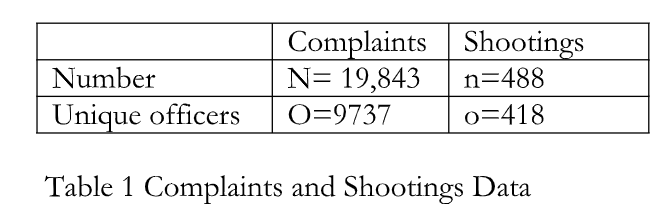
\includegraphics[width=0.4\textwidth]{figs/complaints_shootings_table_0.png}
\caption{table 1}
\end{figure}


In addition, the IPRA dataset reporting police-involved shootings has several
important limitations. Most notably, subsequent analysis by the City of
Chicago’s Office of Inspector General (OIG) found that IPRA did not follow best
practices in reporting use of force. Among other difficulties, IPRA relied on
CPD notifications, and did not independently verify that the Department had
provided all of the required weapons-discharge notifications.  At the same
time, the data appears relatively reliable. The OIG report compared the IPRA
reported shootings to those reported in CPD internal “tactical response
reports.” The comparison found that IPRA’s shooting data from September 2007 to
September 2014, which reported 488 “hit shootings,” had overreported by only
four shootings compared to the CPD tactical response reports, an error rate we
deemed to be within an acceptable range. 

We used IPRA incident-level shooting data to layer shooting events occurring
during the period under study onto the complaint network of co-listed officers
described above. For each shooting event, we recorded the date and location
(street address) of the shooting. We added this information to the complaint
network by adding the shooting event data to the officer-nodes in the network,
and in particular, to the officers who were recorded as having committed the
shootings. 

Fig. 2  Construction of the shooting network. On the left, the complaint network with shooting officers in red; on the right, the resulting shooting network.

In contrast to the complaint network, the shootings network is an event-focused
network. Some officers are involved with more than one shooting. A significant
fraction (86\%, n=358) of officers in the complaint network were associated
with only one shooting. A smaller fraction (12\%, n=51) of officer nodes were
associated with two shootings; 2\% (n=8) were involved in three shootings, and
one officer (Tracey Williams) was involved in five shootings. All of these
shootings are represented in the shootings network. 


\begin{figure}
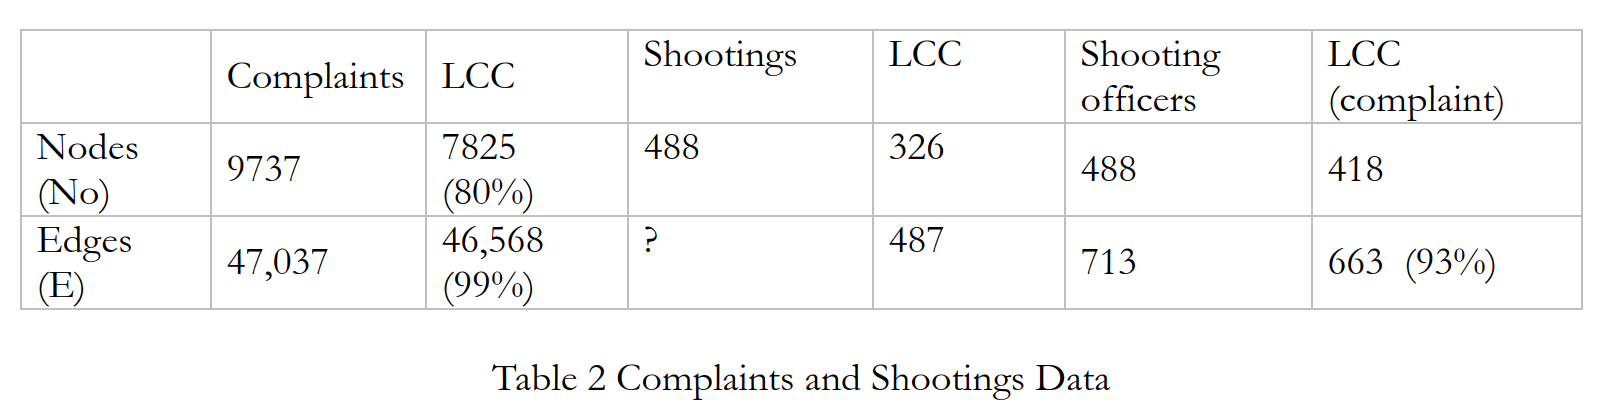
\includegraphics[width=0.4\textwidth]{figs/complaints_shootings_table.png}
\caption{table 2}
\end{figure}



%log_number,officer_name,unique_identifier,incident_date,incident_address,incident_year,specific_day_time


%Complaint_Number,Beat,Location_Code,Address,Street,Apartment,City_State_Zipcode,Incident_Datetime,Complaint_Date,Closed_Date,Full_Address,Investigator_Name,Investigator_Current_Assignment,Investigator_Rank,Investigator_Star,Investigator_Date_Appointed,Accused_Name,Accused_Birth_Yr,Accused_Gender,Accused_Race_Code,Accused_Date_Appointed,Accused_Current_Unit,Accused_Current_Rank,Accused_Star,Accused_Complaint_Category,Accused_Finding,Accused_Recommended_Discipline,Accused_Final_Finding,Accused_Discipline,PO_Witness_Name,PO_Witness_Gender,PO_Witness_Race,PO_Witness_Star,PO_Witness_Birth_Year,PO_Witness_Date_Appointed,Victim_Gender,Victim_Age,Victim_Race_Desc,Complainant_Gender,Complainant_Age,Complainant_Race_Desc

\subsection{Officer covariates}


% the roster data (as of April 2017):
%row_id,gender,race,birth_year,current_age,current_status,appointed_date,rank_no,current_rank,current_unit,unit_description,resignation_date,star1,star2,star3,star4,star5,star6,star7,star8,star9,star10,first_name,first_name_NS,last_name,last_name_NS,middle_initial,middle_initial2,suffix_name,merge,roster_1936-2017_2017-04_ID,UID,old_UID,link_UID

\begin{figure}
\centering
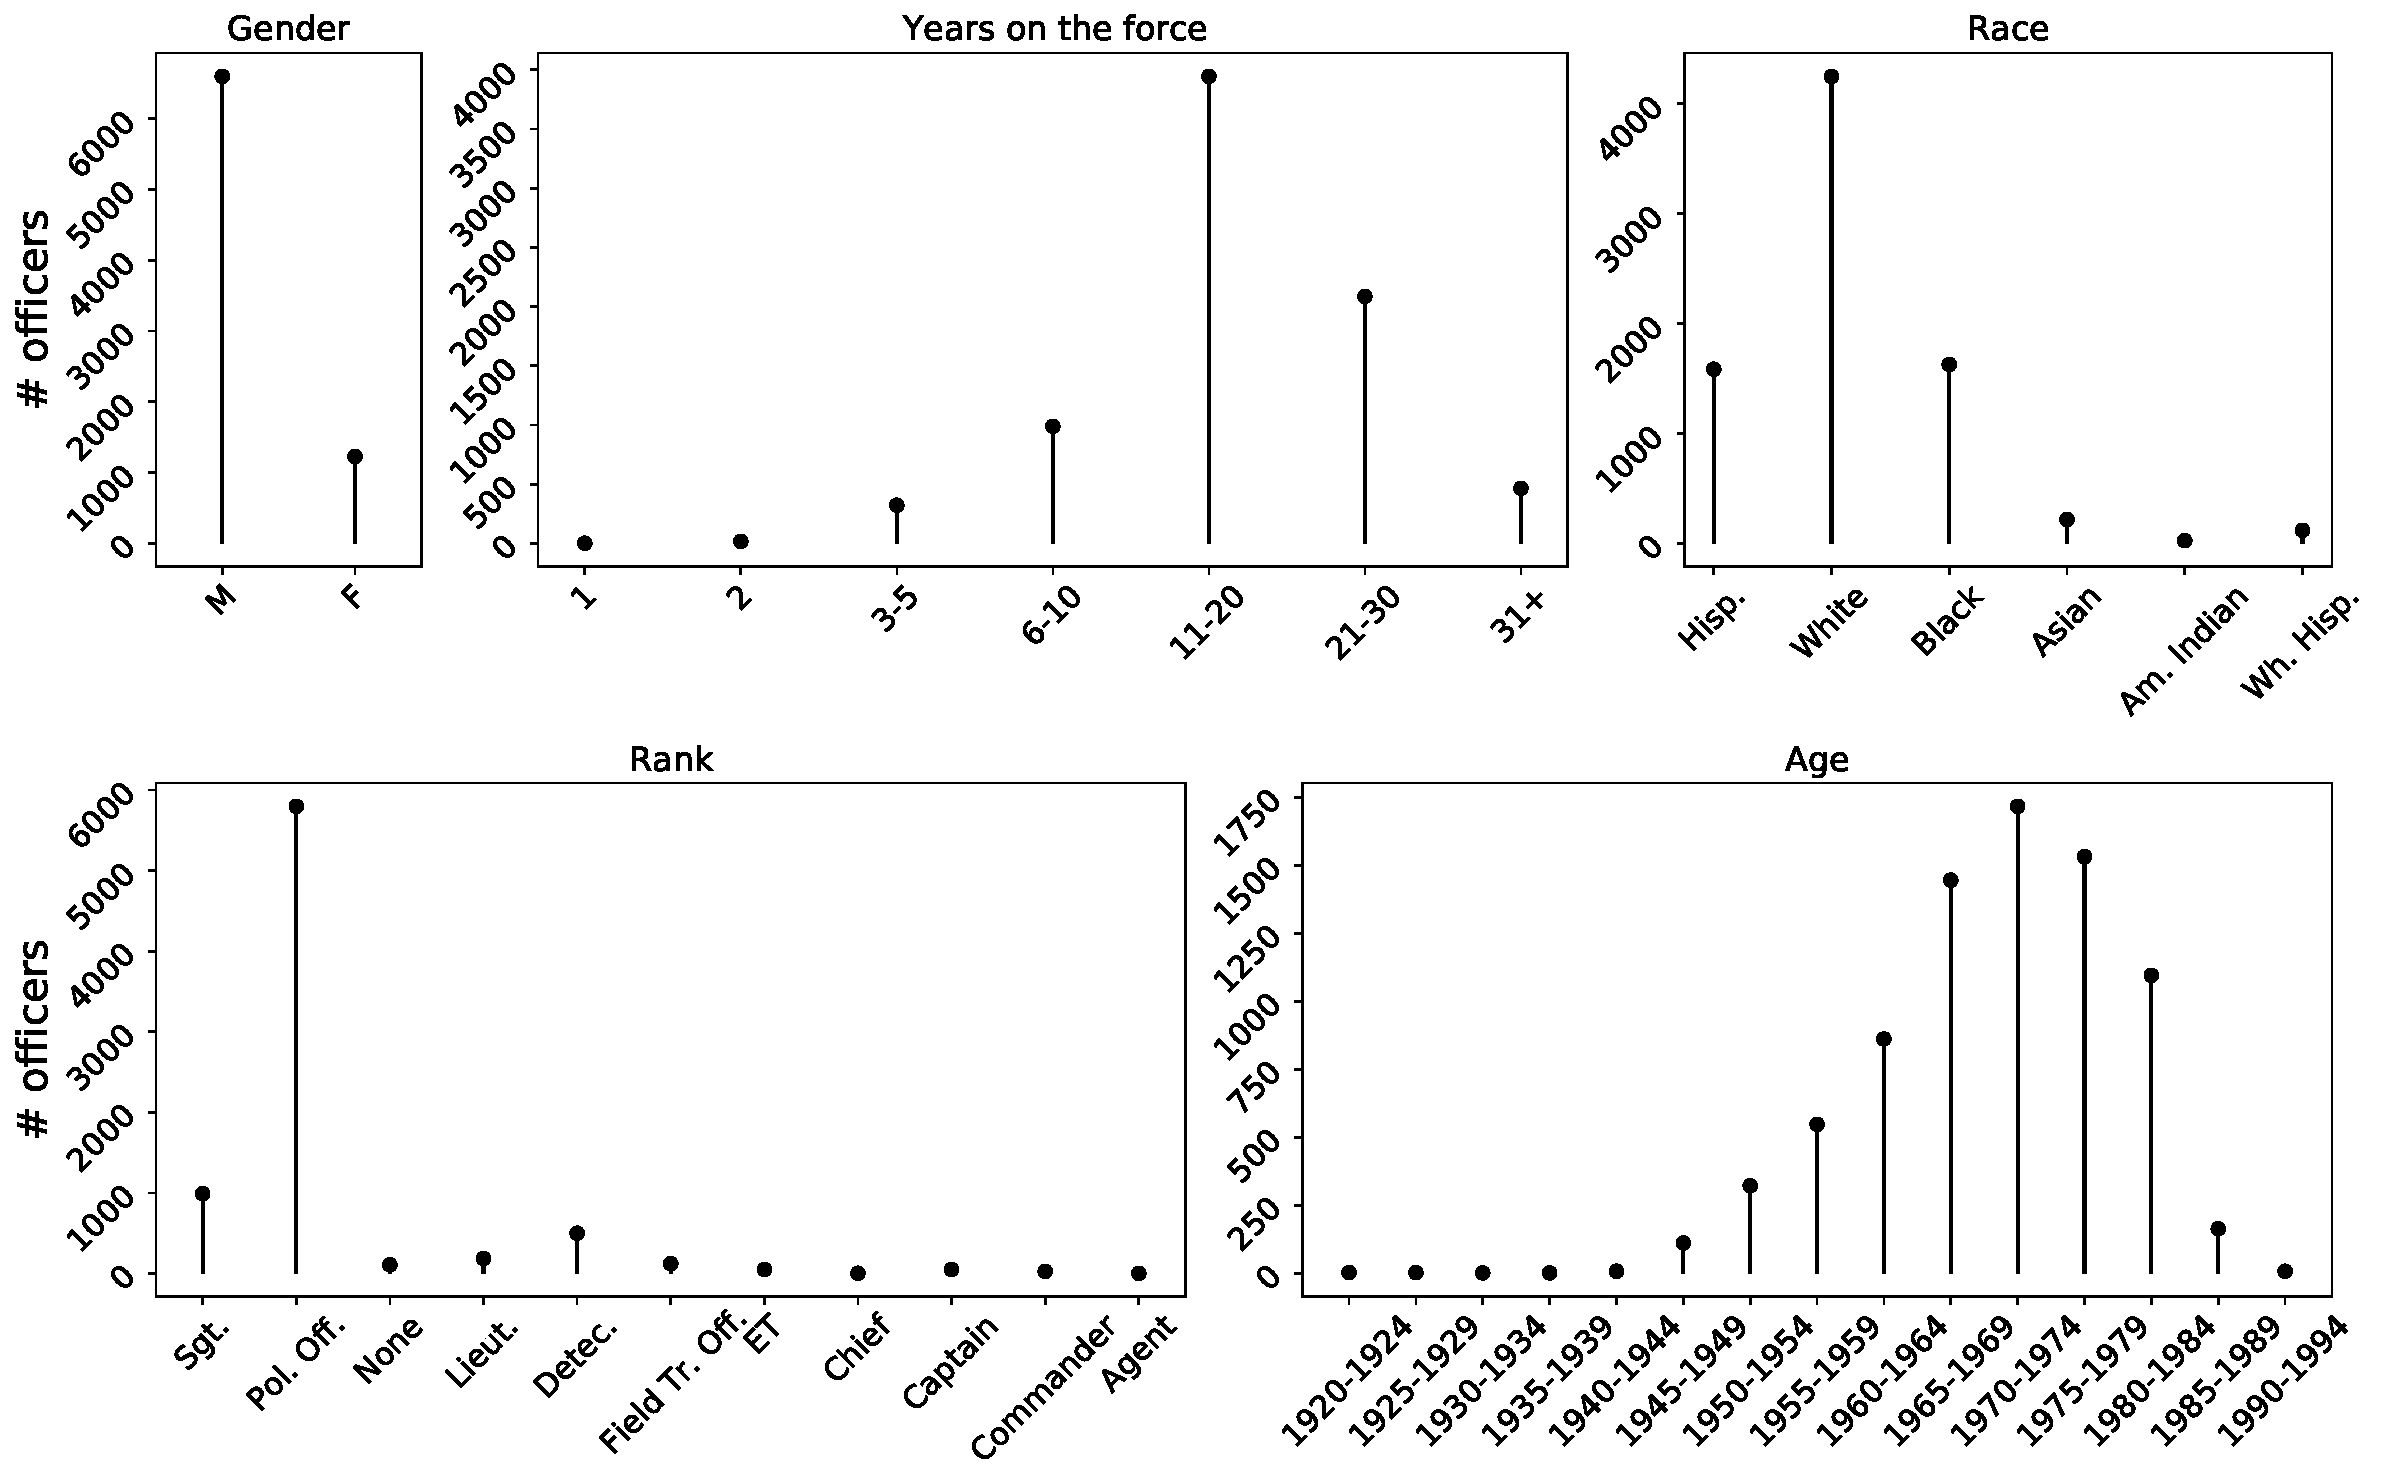
\includegraphics[width=\textwidth]{figs/data_inspection.pdf}
\caption{histograms of officer covariate}\label{fig:histograms}
\end{figure}

\begin{figure}
\centering
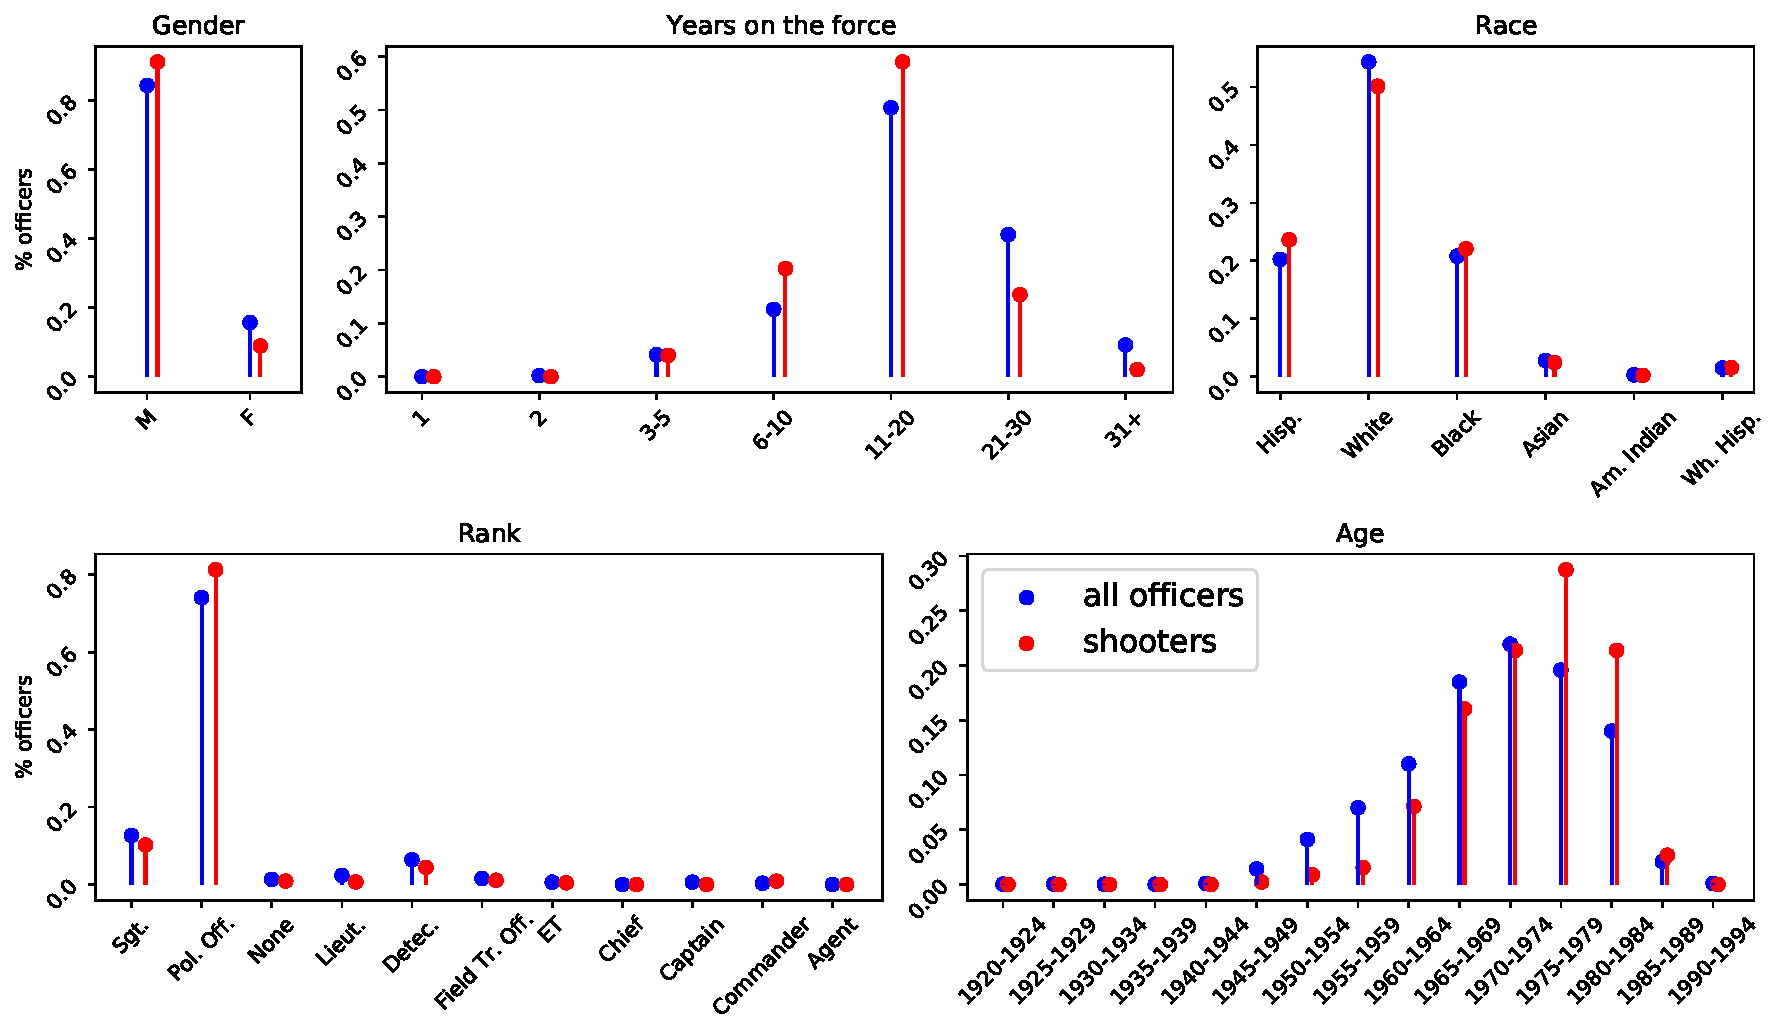
\includegraphics[width=\textwidth]{figs/shooters_relative.pdf}
\caption{histograms of shooter covariate (relative)}\label{fig:shooterhist}
\end{figure}

For each officer, the following information was available in our data: full
name, gender, race, birth date, appointment date, resignation date, rank, badge
number(s), and full unit membership history (including unit number, beginning date, and end date for each membership record).  
We used five of these variables---gender, race, birth date, rank, and number of years on the force since appointment---directly
as covariates in our statistical analyses. 
Figure \ref{fig:histograms} shows the distribution of values for each of these three covariates in the largest
connected component of the officer network. 
As we do not expect an officer's name or badge number to have any additional effect on their likelihood of shooting,
we did not use these variables as covariates. 
The sixth and final covariate for each officer that we considered is their unit membership history.
This section details how we processed each officer's unit membership
history to form a covariate for each officer, and then how we combined this with the previous covariates.

Our data contained a list of 242 unique units with a name and number. After removing
units that were not joined by any officer in the largest connected network component---many of them
old units that no longer exist---179 remained. We separated the units into groups
based on their function, to attempt to ensure a consistent effect on the likelihood of officer shootings in each group. 
The original unit reference data did not contain any actual description of unit function; for those
whose purpose was not clear from the name or whose name was missing entirely, 
we used the following sources to investigate unit function by number:
\begin{itemize}
\item Police directives from \url{http://directives.chicagopolice.org} and \url{https://directives.crimeisdown.com}
\item Investigatory Stop Report (ISR) counts by unit from the CPD annual reports 2017, 2018
\item Tactical Response Report (TRR) counts by unit from the CPD annual reports 2017, 2018
\item Chicago Data Portal crime counts: \url{https://data.cityofchicago.org/Public-Safety/Crimes-2001-to-Present/ijzp-q8t2}
\item Unit mentions in annual reports: \url{https://home.chicagopolice.org/statistics-data/statistical-reports/annual-reports/}
\item Specialized unit information: \url{https://home.chicagopolice.org/about/specialized-units/}
\item Organization charts: \url{https://www.chicago.gov/content/dam/city/depts/cpb/SuperintendentSearch/CPDOrgChart.pdf},
\url{https://home.chicagopolice.org/wp-content/uploads/2020/01/Department-Organization-for-Command-2019-July-19.pdf }
\end{itemize}

The resulting grouping of units is as follows. In total, we grouped the units into 
14 groups, plus an additional extra group for unit numbers appearing in the network whose
function and/or name are unknown. Some units appeared with duplicate numbers to others
(labelled ``dup.'' in the unit tables), but the duplicate name had the same meaning as the original
and did not influence grouping. 
\begin{description}
\item[Low Intensity / Unarmed Officers (49 units, 1 group, Table \ref{tab:desk})] Units
engaging in non-public-facing and
non-criminal-facing activities, units with unarmed officers,
and units performing low-intensity activities {\color{red}as judged by ISR / TRR}.
%
\item[District Units (27 units, 4 groups, Table \ref{tab:district})] Units that
correspond to patrols in the 25 districts\footnote{{\color{red} as of recent;
these change over time. How did we handle this?}} of Chicago. Of these, 25 are district-specific, and
the remaining two are city-wide. Given that Chicago is strongly racially and
economically segregated by district, we decided not to treat all district
patrols as a single unit type in the data, but rather clustered the district
units into 4 groups based on the number of homicides within each district
during the study period using the $k$-means algorithm \cite{xx}.  Figure
\ref{fig:districtclusters} shows the clustering of districts by number of
homicides, and Figure \ref{fig:districtelbow} shows the ``elbow plot'' used
to decide on the number of clusters. 
The two remaining units in this group are the bureau of patrol and
recruit training units; we treated officers in these units as city-wide
patrols, and used the average number of homicides city-wide to cluster these
units.
%
\item[Area Units (33 units, 3 groups, Table \ref{tab:area})] Units that operate within
the 6 areas\footnote{{\color{red} as of recent; these change over time. How did we handle this?}}  of
Chicago.  These include area patrols, youth divisions, gang and narcotics enforcement,
and violent and property crimes. We subdivided the area-based units similarly
to the district-based units due to the strong racial and economic segregation
of the city; in particular, we clustered the area units into 3 groups based on
the number of homicides in the area during the study period using the $k$-means
algorithm \cite{xx}. Figure \ref{fig:areaclusters} shows the clustering of
areas by number of homicides, and Figure \ref{fig:areaelbow} shows the ``elbow plot'' used
to decide on the number of clusters.
%
\item[Detail \& Controlled Zone Security (16 units, 2 groups, Table \ref{tab:controlzone}) ] Units whose officers
provide security of ``controlled zones'' (e.g., airports, courts, construction sites). Of these,
5/11 were labelled ``high/low-intensity'' {\color{red} based on ISR/TRR}.
%
\item[City-Wide Investigations (29 units, 2 groups, Table \ref{tab:citywide})] Units whose officers
perform city-wide detective, investigatory, and enforcement work. 
Of these, 16/13 were labelled ``high/low-intensity'' {\color{red} based on ISR/TRR}.
One unit worth mentioning is the Juvenile Intervention Support Center (JISC); although
we placed this unit in the ``low-intensity'' group, it 
could have equally been sorted into the ``high-intensity'' category, based
on its middling ISR and TRR counts.
%
\item[Special Operations (12 units, 2 groups, Table \ref{tab:specops})] Units whose officers
engage in special operations (e.g., SWAT, mounted, mobile strike force).
Of these, 9/3 were labelled ``high/low-intensity'' {\color{red} based on ISR/TRR}.
%
\item[Unknown (13 units, 1 group, Table \ref{tab:unk})] Units that are labelled as unknown in our dataset, and/or for which
we could not find any credible source of information detailing either the name or purpose of the unit. Given
naming/numbering patterns that are present in the remainder of the data, we hypothesize that units 271--5 are 
area-specific special operations units; but we could not verify this with any existing records. Although unit 45 had
a known label (``district reinstatement''), we could not find any source that described its purpose.

\end{description}



Next, we calculated the fraction of each officer's career spent being a member of
each of these groups. Note that officers can be a member of one or multiple units at the same time, so
these fractions do not necessarily sum to 1. The final ``unit membership'' covariate for each officer
was the vector of these 14 values (all between 0 and 1), one for each unit group.

Finally, we discretized the 6 covariates (gender, race, birth date, rank, number of years on the force since appointment,
and 14 fractions of time spent in each unit group) into bins:
\begin{description}
\item[Gender] 2 values were present in the data: male and female.
\item[Race] 6 values were present in the data: hispanic, white, black, asian/pacific islander, indian, and other. {\color{red} these correct?} 
\item[Birth Date] We grouped birth years together by 5 year intervals, resulting in {\color{red} XX bins}.
\item[Rank] {\color{red}XX values were present in the data: ...}
\item[Years on the Force] We grouped years on the force into 8 bins: 1, 2, 3-5, 6-10, 11-20, 21-30, 31-40, and 40+.
\item[Unit Membership] We discretized all 14 fractions into spacings of 0, 0.1, 0.2, etc. This created $10^{14}$ bins.
\end{description}
Combining all of these covariates, each officer was described by one of $xx$ unique values. Only officers with precisely
the same value were eligible to be swapped in the permutation test. 

Figure \ref{xx} shows the occupancy of bins

{\color{red} there were also units that appeared in our dataset but no officer was a recorded member of them in the network? LCC? here's the list of those}



\begin{figure}[h!]
\centering
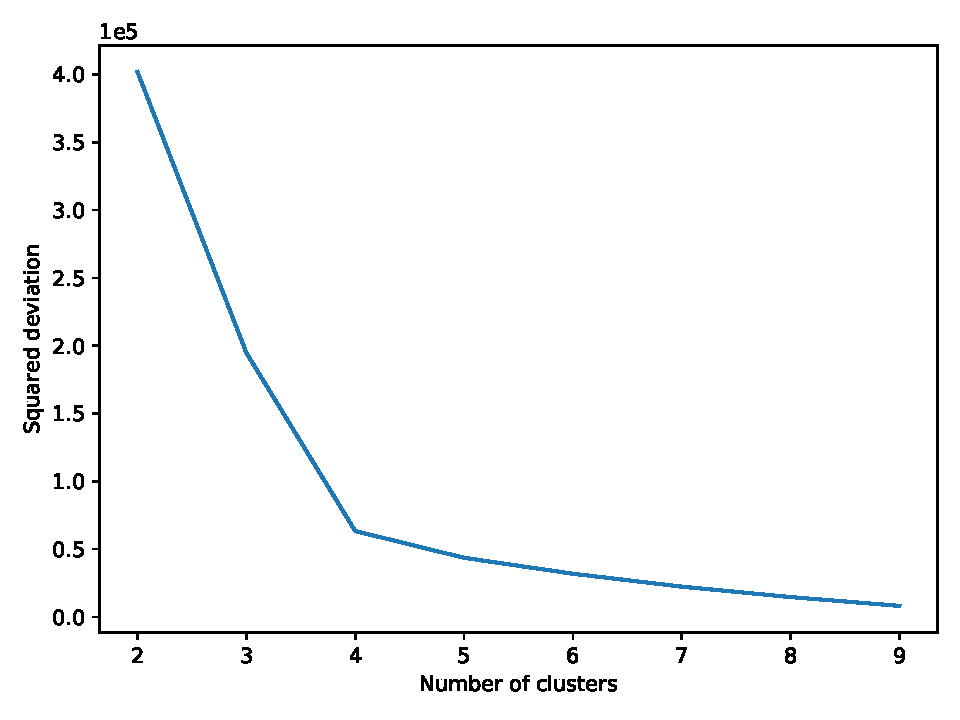
\includegraphics[width=0.75\textwidth]{figs/elbow-districts.pdf}
\caption{}\label{fig:districtelbow}
\end{figure}

\begin{figure}[h!]
\centering
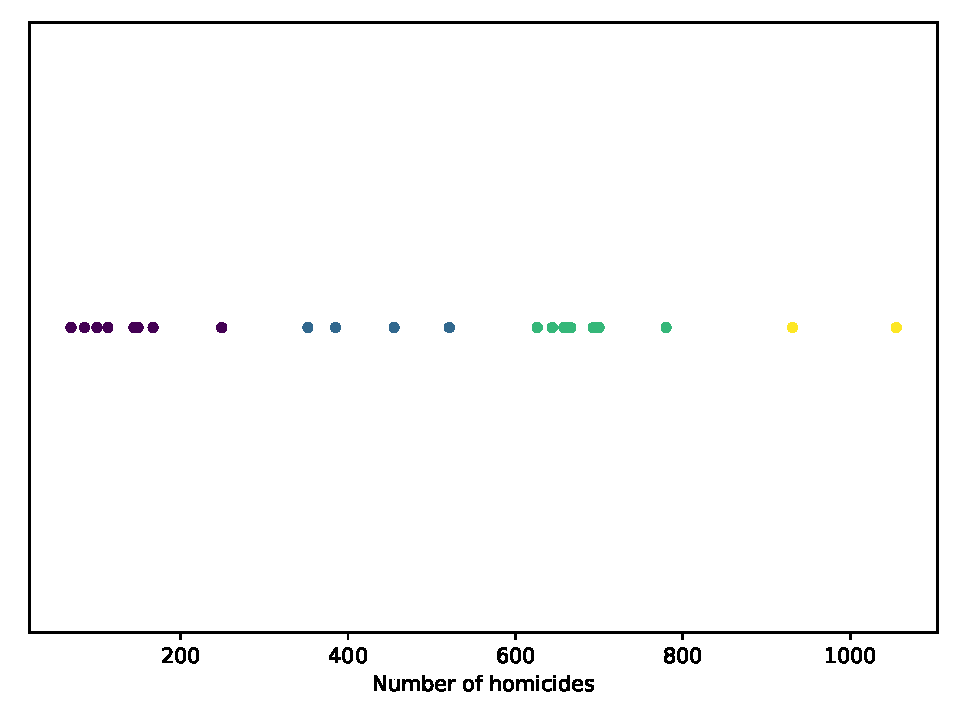
\includegraphics[width=0.75\textwidth]{figs/clusters-districts.pdf}
\caption{}\label{fig:districtclusters}
\end{figure}

\begin{figure}[h!]
\centering
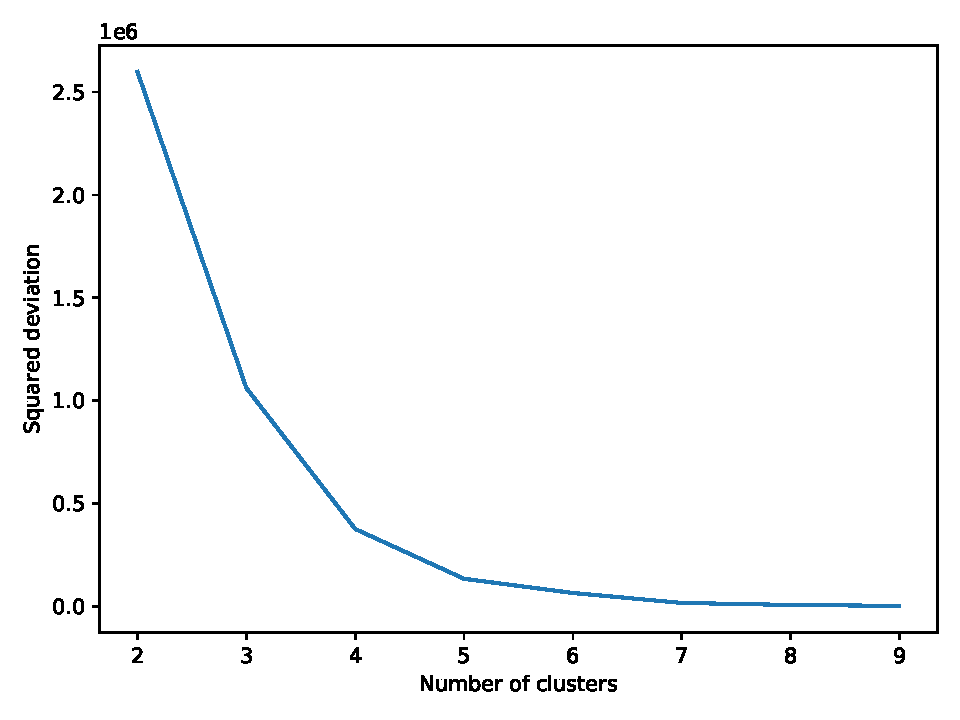
\includegraphics[width=0.75\textwidth]{figs/elbow-areas.pdf}
\caption{}\label{fig:areaelbow}
\end{figure}

\begin{figure}[h!]
\centering
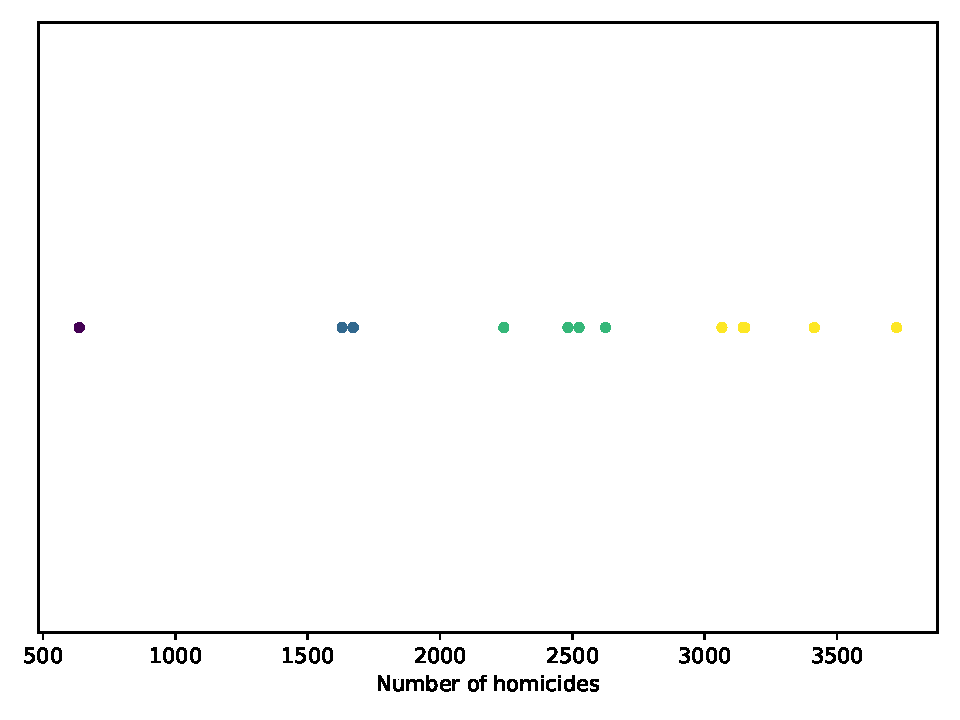
\includegraphics[width=0.75\textwidth]{figs/clusters-areas.pdf}
\caption{}\label{fig:areaclusters}
\end{figure}




\begin{table}
\tiny
\centering
\caption{}\label{tab:desk}
\begin{tabular}{|ll|}
\hline
Type: &	\textbf{Very Low Intensity \& Unarmed Officers} \\
\hline
Unit \# &	Unit Name \\
\hline
26	&Executive Officers Unit\\
86	&OEC-Police Dispatch\\
102	&Office Of News Affairs\\
111	&Office Of The Superintendent\\
112	&Bureau Of Professional Standards\\
114	&Legal Affairs Section\\
115	&CAPS Project Office\\
115	&Crime Control Strategies Section\\
116	&Deployment Operations Center\\
119	&Office Of International Relations\\
120	&Bureau Of Support Services\\
121	&Bureau Of Internal Affairs\\
123	&Human Resources Division\\
125	&Information Services Division\\
127	&Research And Development Division\\
128	&Professional Counseling Division\\
129	&Management And Labor Affairs Section\\
130	&Bureau Of Organizational Development\\
130	&Technology And Records Group\\
130	&Bureau Of Staff Services\\
163	&Records Inquiry Section\\
167	&Evidence And Recovered Property Section\\
169	&Police Documents Section\\
170	&CT \& ID Administration\\
172	&Equipment And Supply Section\\
175	&Telecommunications Unit\\
176	&Communication Operations Unit\\
214	&Freedom Of Information Section\\
216	&Deputy Chief Central Control Group\\
179	&Reproduction And Graphic Arts Section\\
231	&Medical Section\\
159	&Gun Registration\\
157	&Pub Housing Div Adm\\
601	&Det Div Admin.\\
944	&Cops Grant Recr Trng\\
165	&Field Inquiry Section\\
161	&General Support Division\\
139	&Asst Superintendent-Law Enforcement Operations (dup. CAPS)\\
140	&Office Of The First Deputy Superintendent\\
376	&Alternate Response Section\\
136	&Special Events Unit\\
166	&Field Services Section\\
126	&Inspection Division\\
147	&Senior Citizen Services\\
154	&Traffic Safety And Training\\
168	&Auto Pound Section\\
441	&Special Activities Section\\
135	&Chicago Alternative Policing Strategy (CAPS) Division\\
136	&CAPS\\
\hline
\end{tabular}
\end{table}



\begin{table}
\tiny
\centering
\caption{}\label{tab:district}
\begin{tabular}{|llll|}
\hline
Type: &	\textbf{District-Specific Units}  & &\\
\hline
Unit \# &Unit Name & Homicides & Cluster  \\
\hline
1	&District 001	&100	&0\\
2	&District 002	&455	&1\\
3	&District 003	&662	&2\\
4	&District 004	&693	&2\\
5	&District 005	&658	&2\\
6	&District 006	&780	&2\\
7	&District 007	&931	&3\\
8	&District 008	&644	&2\\
9	&District 009	&666	&2\\
10	&District 010	&700	&2\\
11	&District 011	&1055	&3\\
12	&District 012	&385	&1\\
13	&District 013	&385	&1\\
14	&District 014	&249	&0\\
15	&District 015	&626	&2\\
16	&District 016	&85	&0\\
17	&District 017	&149	&0\\
18	&District 018	&113	&0\\
19	&District 019	&144	&0\\
20	&District 020	&69	&0\\
21	&District 021	&455	&1\\
22	&District 022	&352	&1\\
23	&District 023	&144	&0\\
24	&District 024	&167	&0\\
25	&District 025	&521	&1\\
142	&Bureau Of Patrol	&447.52	&1\\
44	&Recruit Training Section	&447.52	&1\\
\hline
\end{tabular}
\end{table}



\begin{table}
\tiny
\centering
\caption{}\label{tab:area}
\begin{tabular}{|llll|}
\hline
Type: &	\textbf{Area-Specific Units}  & &\\
\hline
Unit \# &Unit Name & Homicides & Cluster  \\
\hline
71	&Youth Division Area1	&1672	&0\\
72	&Youth Division Area2	&2483	&1\\
73	&Youth Division Area3	&2241	&1\\
74	&Youth Division Area4	&2525	&1\\
75	&Youth Division Area5	&1630	&0\\
76	&Youth Division Area6	&637	&0\\
211	&Bureau Of Patrol - Area Central&3725	&2\\
212	&Bureau Of Patrol - Area South	&3414	&2\\
213	&Bureau Of Patrol - Area North	&3065	&2\\
214	&Deputy Chief - Area 4 (dup. Free. Of Info. Divn)&2625	&1\\
62	&Area 2 Pat Narc Prog	&2483	&1\\
63	&Area 3 Pat Narc Prog	&2241	&1\\
65	&Area 5 Pat Narc Prog	&1630	&0\\
66	&Area 6 Pat Narc Prog	&637	&0\\
311	&Gang Enforcement - Area Central&3151	&2\\
312	&Gang Enforcement - Area South	&3145	&2\\
313	&Gang Enforcement - Area North	&637	&0\\
314	&Gang Section - Area 4	&2625	&1\\
315	&Gang Section - Area 5	&1630	&0\\
612	&Violent Crimes DDA 1	&3151	&2\\
610	&Detective Area - Central	&3725	&2\\
620	&Detective Area - South	&3414	&2\\
621	&Prop Crimes DDA 2	&3145	&2\\
622	&Violent Crimes DDA 2	&3145	&2\\
630	&Detective Area - North	&3065	&2\\
631	&Prop Crimes DDA 3	&637	&0\\
632	&Violent Crimes DDA 3	&637	&0\\
640	&Detective Section - Area 4	&2625	&1\\
641	&Prop Crimes DDA 4	&2625	&1\\
642	&Violent Crimes DDA 4	&2625	&1\\
650	&Detective Section - Area 5	&1630	&0\\
651	&Prop Crimes DDA 5	&1630	&0\\
652	&Violent Crime DDA 5	&1630	&0\\
\hline
\end{tabular}
\end{table}



\begin{table}
\tiny
\centering
\caption{}\label{tab:controlzone}
\begin{tabular}{|ll|}
\hline
Type:	&\textbf{Detail \& Controlled Zone Security - High Intensity}\\ 
\hline
Unit \#	&Unit Name \\
\hline
704	&Transit Security Unit\\	
701	&Public Transportation Section \\
50	&Airport Law Enforcement Section - North \\ 
51	&Airport Law Enforcement Section - South \\
171	&Central Detention Unit	\\ 
\hline
Type:	&\textbf{Detail \& Controlled Zone Security - Low Intensity}\\ 
\hline
Unit \#	&Unit Name \\
\hline
143	&Court Section (dup .District Law)\\
261	&Court Section\\
284	&Admin School Securit\\
541	&FOP Detail\\
542	&Detached Services - Goverment Security\\
543	&Detached Services - Miscellaneous Detail\\
276	&OEC - Detail Section\\
57	&Traffic Section Detail Unit (dup. Detail Unit)\\
151	&Traffic Enforcement\\
152	&Loop Traffic Unit\\
145	&Traffic Section\\
\hline
\end{tabular}
\end{table}


\begin{table}
\tiny
\centering
\caption{}\label{tab:citywide}
\begin{tabular}{|ll|}
\hline
Type:	&\textbf{City-wide Investigations - High Intensity}\\ 
\hline
Unit \#	&Unit Name \\
\hline
189	&Narcotics Division\\
91	&Narc Special Enforce\\
92	&Narc General Enforce\\
156	&Gang Crime Section\\
393	&Gang Enforcement Division\\
188	&Bureau Of Organized Crime\\
193	&Gang Investigation Division\\
192	&Vice \& Asset Forfeiture Division\\
196	&Asset Forfeiture Investigation Section \\
740	&G/C Unit West\\
760	&G/C Unit North\\
710	&G/C Unit South\\
765	&Public Housing North\\
715	&Public Housing South\\
132	&Preven \& Neigh Div\\
606	&Central Investigations Division\\
\hline
Type:	&\textbf{City-wide Investigations - Low Intensity}\\
\hline
Unit \#	&Unit Name \\
\hline
79	&Special Investigations Unit\\
180	&Bureau Of  Detectives\\
184	&Youth Investigation Division\\
608	&Major Accident Investigation Unit\\
602	&Central Auto Theft\\
603	&Arson Section\\
603	&Bomb And Arson Division\\
384	&Juvenile Intervention Support Center (JISC)\\
191	&Intelligence Section\\
277	&Forensic Services Evidence Technician Sectn\\
377	&Forensic Services Unit - ET North\\
477	&Forensic Services Unit - ET South\\
177	&Forensic Services Division\\
\hline
\end{tabular}
\end{table}


\begin{table}
\tiny
\centering
\caption{}\label{tab:specops}
\begin{tabular}{|ll|}
\hline
Type:	&\textbf{Special Operations - High Intensity}\\ 
\hline
Unit \#	&Unit Name \\
\hline
55	&Mounted Unit\\
58	&Spec Func Canine\\
341	&Canine Unit\\
353	&Special Weapons And Tactics (SWAT) Unit\\
153	&Mobile Strike Force (dup. Special Functions Support Unit)\\
141	&Special Functions Division\\
146	&Canine Unit\\
241	&Troubled Building Unit\\
253	&Targeted Response Unit\\
\hline
Type:	&\textbf{Special Operations - Low Intensity}\\
\hline
Unit \#	&Unit Name \\
\hline
59	&Marine Operations Unit\\
442	&Bomb Squad\\
124	&Education And Training Division\\
\hline
\end{tabular}
\end{table}


\begin{table}
\tiny
\centering
\caption{}\label{tab:unk}
\begin{tabular}{|ll|}
\hline
Type: &	\textbf{Unknown} \\
\hline
Unit \# &	Unit Name \\
\hline
45  & District Reinstatement \\
52  & Unknown\\
54  & Unknown\\
56  & Unknown\\
64  & Unknown\\
661 & Unknown\\
720 & Unknown\\
271 & Unknown (Special Funcs Area 1?)\\
272 & Unknown (Special Funcs Area 2?)\\
273 & Unknown (Special Funcs Area 3?)\\
274 & Unknown (Special Funcs Area 4?)\\
275 & Unknown (Special Funcs Area 5?)\\
911 & Unknown \\
\hline
\end{tabular}
\end{table}




{\color{red}
\paragraph{Questions:}
\begin{itemize}
\item for years on the force -- this is appointment date minus what?  \tbo{end of study period minus appointment date}
\item what did we do with officers in the LCC who did not match?
\item did we include the UNK bins? how? -- yes, the unk fraction is treated as another "component" in the vector covariate
\item how did we deal with changing areas over time? changing districts?
\item 4 clusters in area unit plot, but only 3 unit bins
\end{itemize}
}

\begin{figure}[h!]
\centering
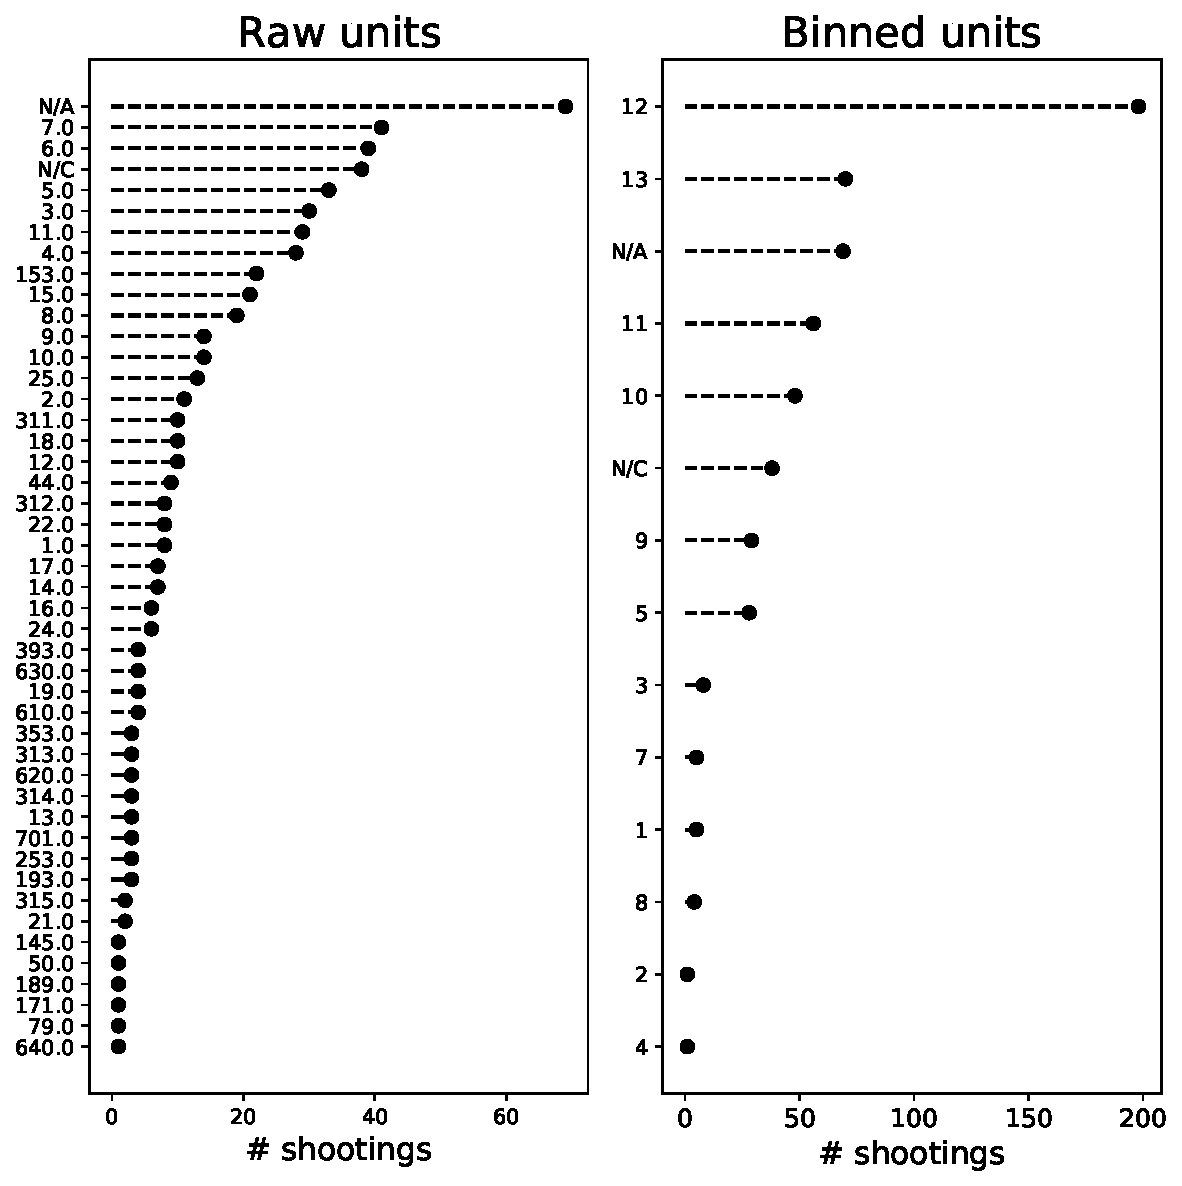
\includegraphics[width=0.75\textwidth]{figs/unit_plots.pdf}
\caption{}\label{fig:unitplots}
\end{figure}

Figure \ref{fig:unitplots} shows the number of shooting events
performed by officers in each unit and each unit bin during the study
period. To construct this figure, note that there are three
situations for each shooting event:
\begin{itemize}
\item The shooting officer is not present in the largest connected component of our network. 
These events are not included in the study, but we show them here labelled
``N/C'' (not counted). There are 38 such shooting events by 35/484 unique officers.
\item The shooting officer is present in the largest connected component but we could
not find a positive match for the officer in the roster (which has the unit history). 
These events are labelled ``N/A'' (not available). There are 69 such shooting events
by 57/484 unique officers.
\item The shooting officer is present in the largest connected component and there is
a positive match in the roster. There are 452 such shooting events by 392/484 unique officers.
Note that it is possible that a shooting officer is a member of multiple units simultaneously;
in this case, we add +1 to the shooting event counts for every unit the officer was a member of
at the time of shooting. But there is only one shooting event with such a situation, % Thomas Dineen 
where the officer was a member of both units 15 and 153.
\end{itemize}



\bibliographystyle{unsrtnat}
\bibliography{references}

\section*{Checklist}

%%% BEGIN INSTRUCTIONS %%%
The checklist follows the references.  Please
read the checklist guidelines carefully for information on how to answer these
questions.  For each question, change the default \answerTODO{} to \answerYes{},
\answerNo{}, or \answerNA{}.  You are strongly encouraged to include a {\bf
justification to your answer}, either by referencing the appropriate section of
your paper or providing a brief inline description.  For example:
\begin{itemize}
  \item Did you include the license to the code and datasets? \answerYes{See Section~\ref{gen_inst}.}
  \item Did you include the license to the code and datasets? \answerNo{The code and the data are proprietary.}
  \item Did you include the license to the code and datasets? \answerNA{}
\end{itemize}
Please do not modify the questions and only use the provided macros for your
answers.  Note that the Checklist section does not count towards the page
limit.  In your paper, please delete this instructions block and only keep the
Checklist section heading above along with the questions/answers below.
%%% END INSTRUCTIONS %%%

\begin{enumerate}

\item For all authors...
\begin{enumerate}
  \item Do the main claims made in the abstract and introduction accurately reflect the paper's contributions and scope?
    \answerTODO{}
  \item Did you describe the limitations of your work?
    \answerTODO{}
  \item Did you discuss any potential negative societal impacts of your work?
    \answerTODO{}
  \item Have you read the ethics review guidelines and ensured that your paper conforms to them?
    \answerTODO{}
\end{enumerate}

\item If you are including theoretical results...
\begin{enumerate}
  \item Did you state the full set of assumptions of all theoretical results?
    \answerTODO{}
	\item Did you include complete proofs of all theoretical results?
    \answerTODO{}
\end{enumerate}

\item If you ran experiments (e.g. for benchmarks)...
\begin{enumerate}
  \item Did you include the code, data, and instructions needed to reproduce the main experimental results (either in the supplemental material or as a URL)?
    \answerTODO{}
  \item Did you specify all the training details (e.g., data splits, hyperparameters, how they were chosen)?
    \answerTODO{}
	\item Did you report error bars (e.g., with respect to the random seed after running experiments multiple times)?
    \answerTODO{}
	\item Did you include the total amount of compute and the type of resources used (e.g., type of GPUs, internal cluster, or cloud provider)?
    \answerTODO{}
\end{enumerate}

\item If you are using existing assets (e.g., code, data, models) or curating/releasing new assets...
\begin{enumerate}
  \item If your work uses existing assets, did you cite the creators?
    \answerTODO{}
  \item Did you mention the license of the assets?
    \answerTODO{}
  \item Did you include any new assets either in the supplemental material or as a URL?
    \answerTODO{}
  \item Did you discuss whether and how consent was obtained from people whose data you're using/curating?
    \answerTODO{}
  \item Did you discuss whether the data you are using/curating contains personally identifiable information or offensive content?
    \answerTODO{}
\end{enumerate}

\item If you used crowdsourcing or conducted research with human subjects...
\begin{enumerate}
  \item Did you include the full text of instructions given to participants and screenshots, if applicable?
    \answerTODO{}
  \item Did you describe any potential participant risks, with links to Institutional Review Board (IRB) approvals, if applicable?
    \answerTODO{}
  \item Did you include the estimated hourly wage paid to participants and the total amount spent on participant compensation?
    \answerTODO{}
\end{enumerate}

\end{enumerate}


\appendix



\section{Datasheet}\label{sec:datasheet}

This section provides a datasheet \cite{Gebru18} for the dataset repository.

\subsection{Motivation}

\paragraph{For what purpose was the dataset created?}
The original raw data files were sought by J.~Kalven, a journalist in the City
of Chicago, as part of his investigation into police abuse. After the original
FOIA requests and legal case, the non-profit Invisible Institute (\url{https://invisible.institute}) 
began to collaborate with Kalven and the University of Chicago's Mandel Legal Aid Clinic
to follow up on earlier FOIA requests and to file new ones. The data disclosed
in response to these earlier and now ongoing FOIA requests were made available
online as part of the Citizens Police Data Project.

\paragraph{Who created the dataset, and on behalf of which entity?}
The Chicago Police Department (CPD), Civilian Office of Police Accountability
(COPA), and the City of Chicago produced the raw data files in response to FOIA
requests. The raw data were curated and released publicly by the Invisible
Institute and its collaborators. The cleaned and linked data were produced
as part of research by the authors of this document.

\paragraph{Who funded the creation of the dataset?}
The acquisition of the original raw data was funded by the Invisible Institute.

\subsection{Composition}

\paragraph{What do the instances that comprise the dataset represent?}
There are multiple types of instance in this data. 
\begin{itemize}
\item Officer: information about an individual police officer
\item Unit assignment: a single unit assignment for an officer
\item Complaint: a complaint filed against a police officer, either internally or by a civilian
\item Tactical Response Report: a form that an officer is required to fill out after their response requires use of force
\item Award request: a request to grant an award to an officer
\item Salary: a record of an officer's salary, pay grade, and position across multiple years
\end{itemize}

\paragraph{How many instances are there in total (of each type)?}
There are roughly 35,000 unique officers in the cleaned roster appearing in roughly 130,000 profiles throughout the data,
730,000 award request records,
194,000 salary records,
108,000 unit assignment records,
109,000 complaints,
and 10,500 tactical response reports.

\paragraph{Does the dataset contain all possible instances or is it a sample of instances from a larger set?}
This data contains information regarding all sworn officers in the Chicago Police Department / City of Chicago
databases for the stated date ranges (which differ for each source of raw data).

\paragraph{What data does each instance consist of?}
\begin{itemize}
\item Officer: officer unique ID, race, gender, age, appointment date, resignation date, badge number(s), position title(s)
\item Unit assignment: officer unique ID, start date, end date, unit number
\item Complaint: complaint ID, involved officer IDs, allegation, result of the investigation, resulting sanction (where available)
\item Tactical Response Report: report ID, event location, date, and time, environmental conditions, who was notified, weapons discharged, weapon information, subject demographic information 
\item Award Request: awardee unique ID, requester, request date, award reference number, award type, request tracking number, incident dates, ceremony date
\item Salary: officer unique ID, salary, position title, pay grade, year
\end{itemize}

\paragraph{Is there a label or target associated with each instance?}
Not explicitly. However, labels could be constructed from the data 
that exists. For example, one could aggregate complaints to produce
an integer ``number of complaints'' for each officer in the data,
and use that as the response variable in a prediction task.

\paragraph{Is any information missing from individual instances?}
In the original raw data files, missing data (of all fields) is quite common.
In the cleaned and linked data files, we are able to aggregate multiple profiles
of a single officer appearing throughout the data to ``fill in the gaps,'' although
this process is not perfect and there are still missing entries.

\paragraph{Are relationships between individual instances made explicit?}
In the raw data, no. In the cleaned data, we provide a unique officer
identification that enables linking the activities and records regarding
individual officers across datasets. There is no relational data (i.e., network edges)
explicitly contained in the data. However, it is possible to use the data
to construct a network, e.g., by linking officers co-listed on complaints.

\paragraph{Are there recommended data splits?}
No.

\paragraph{Are there any errors, sources of noise, or redundancies in the dataset?}
There are redundancies in the raw data, but these are removed by our cleaning and linking procedure.
Errors, inconsistencies, and missing data are also present in the raw data; our cleaning and linking
resolves much of these issues. However, per \cref{sec:analysis}, the officer database is
likely to be incomplete prior to roughly 1980 (as officers were added to the database only gradually over time).

\paragraph{Is the dataset self-contained, or does it rely on external resources?}
The dataset is self-contained: the raw data itself is stored in the \url{raw/} folder of the repository 
(with links to the external source files for reference), 
and the cleaned/linked data is produced by the source code in the repository.

\paragraph{Does the dataset contain data that might be considered confidential?}
No; all of this data was publicly released as part of FOIA requests. 
Confidential data (e.g., relating to under cover officers) was withheld 
by the Chicago Police Department.

\paragraph{Does the dataset contain data that, if viewed directly, might be offensive, insulting, or threatening?}
No.

\paragraph{Does the dataset relate to people?} 
Yes; it contains records relating to police officers in the Chicago Police Department.

\paragraph{Does the dataset identify any subpopulations?}
Yes; officer records include race, gender, age, appointment date, unit history, badge numbers, position title,
salary, awards, complaints, and tactical response reports. Subpopulations of officers can be constructed
using these fields.

\paragraph{Is it possible to identify individuals?}
Yes; detailed information is available that could be used to identify individual officers.

\paragraph{Does the dataset contain data that might be considered sensitive in any way?}
The data contains a coarse categorization of racial origins of officers.

\subsection{Collection Process}

\paragraph{How was the data associated with each instance acquired?}
The raw data were obtained via FOIA requests to the City of Chicago and Chicago Police Department.

\paragraph{What mechanisms or procedures were used to collect the data?}
The raw data were obtained via FOIA requests to the City of Chicago and Chicago Police Department.

\paragraph{If the data are a sample from a larger set, what was the sampling strategy?}
Not applicable. 

\paragraph{Who was involved in the data collection process and how were they compensated?}
Journalists in collaboration with the Invisible Institute were responsible for filing
the FOIA requests, and officials within the Chicago Police Department and City of Chicago were responsible
for providing data in response to those requests. It is not known explicitly whether or how 
either party was compensated.

\paragraph{Over what timeframe was the data collected?}
The earliest releases per FOIA request occurred in 2016, and continue to occur
as more FOIA requests are filed. The raw data itself pertain to records from the CPD
dating back to the mid 20th century. The roster data covers the period up
to 2018. The awards data pertains to records from 1967 to 2019.
The salary data pertains to the years 2002 to 2017. The unit history data covers records up
to 2016. The complaints data pertains to records from 1967 to 2016. The tactical response 
report data pertains to records from 2004 to 2017.

\paragraph{Were any ethical review processes conducted?}
It is unknown whether the CPD conducted any ethical review processes prior to the release
of the raw data. No ethical review process was conducted prior to the activities
involved in the present repository, i.e., cleaning the publicly available data.

\paragraph{Does the dataset relate to people?}
Yes; it contains detailed records regarding the activities of police officers in the City of Chicago.

\paragraph{Did you collect the data from the individuals directly, or obtain it via third parties?}
The raw data was acquired from public links provided by the Invisible Institute (\url{https://invisible.institute}).
The Invisible Institute acquired the data through FOIA requests made to the CPD and the City of Chicago.

\paragraph{Were the individuals notified about the data collection?}
It is unknown whether the individual officers were notified by the CPD when the raw data was released. 

\paragraph{Did the individuals in question consent to the collection and use of their data?}
Not explicitly. The Chicago Police Department was compelled by law to produce these records per FOIA requests.

\paragraph{If consent was obtained, were the consenting individuals provided with a mechanism to revoke their consent in the future or for certain uses?}
Not applicable.

\paragraph{Has analysis of the potential impact of the dataset and its use on data subjects been conducted?}
Not known.

\subsection{Preprocessing and cleaning}

\paragraph{Was any preprocessing of the data done?}
Yes; the main section of this documentation provides details the cleaning and linking of the raw
data resulting from FOIA requests made to the City of Chicago.

\paragraph{Was the ``raw'' data saved in addition to the cleaned data?}
Yes; the raw data is available in the \url{raw/} folder in the repository.

\paragraph{Is the software used to clean the data available?}
Yes; the source for cleaning and linking is provided in the \url{src/} folder in the repository.

\subsection{Uses}

\paragraph{Has the dataset been used for any tasks already?}
Not the newly cleaned and linked version.
The raw data itself has been used previously; see \cref{sec:discussion} for details.

\paragraph{Is there a repository that links to any or all papers that use the dataset?}
Not that the authors of this work are aware of.

\paragraph{What (other) tasks could the dataset be used for?}
This data set has a rich variety of possible uses; for example,
network analysis (and in particular, analysis of dynamic events occurring on networks)
and predictive regression/classification. See \cref{sec:discussion} for more details.

\paragraph{Is there anything about the composition of the dataset or the way it was collected and cleaned that might impact future uses?}
Yes; the data are less reliable in earlier years (e.g., pre-1980). See \cref{sec:analysis} for more details.

\paragraph{Are there tasks for which the dataset should not be used?}
This data should not be used to single out, study, or identify individual officers.

\subsection{Distribution}

\paragraph{Will the dataset be distributed to third parties outside of the entity on behalf of which the dataset was created?}
Yes, the data is publicly available.

\paragraph{How will the dataset be distributed?}
It is available on GitHub at \url{https://github.com/chicago-police-violence/data}.
Release versions will be marked using the ``release'' feature on GitHub.

\paragraph{When will the dataset be distributed?}
It is currently publicly accessible.

\paragraph{Will the dataset be distributed under a copyright, other IP license, or terms of use?}
Yes; the source code is released under the MIT license, and the data output by the cleaning code is released under the Creative Commons 4.0 BY-NC-SA license.

\paragraph{Have any third parties imposed IP-based or other restrictions on the data associated with the instances?}
No.

\paragraph{Do any export controls or other regulatory restrictions apply to the data?}
No.

\subsection{Maintenance}

\paragraph{Who is supporting/hosting/maintaining the dataset?}
The repository will be hosted on GitHub. As of August 2021, the repository
owners are Thibaut Horel, Trevor Campbell, and Lorenzo Masoero, but ownership
may change over time.

\paragraph{How can the data owner/curator be contacted?}
Issue threads on GitHub are the primary channel of contact for the repository maintainers.

\paragraph{Is there an erratum?}
Not as of yet. For each major release version, notes will be included and
hosted in the repository that will detail cleaning/linking errors that have been fixed.

\paragraph{Will the dataset be updated?}
The original raw source data from FOIA requests will not be modified. More raw
data files may be added over time corresponding to new FOIA requests. The data
cleaning and linking code will be edited over time to fix errors; release
versions will be clearly marked on GitHub. There is no set schedule for updates.

\paragraph{If the dataset relates to people, are there applicable limits on the retention of data associated with the instances?}
No; this data was released per FOIA requests and is in the public domain.

\paragraph{Will older versions of the dataset continue to be supported/hosted/maintained?}
Yes; a full version-controlled history of the project exists on GitHub.

\paragraph{If others want to extend/augment/build on/contribute to the dataset, is there a mechanism for them to do so?}
Yes; the repository for the dataset is hosted on GitHub, where pull requests are a usual channel for external contribution.


\section{Additional summary figures}\label{sec:additional_figs}

\begin{figure}[h] 
	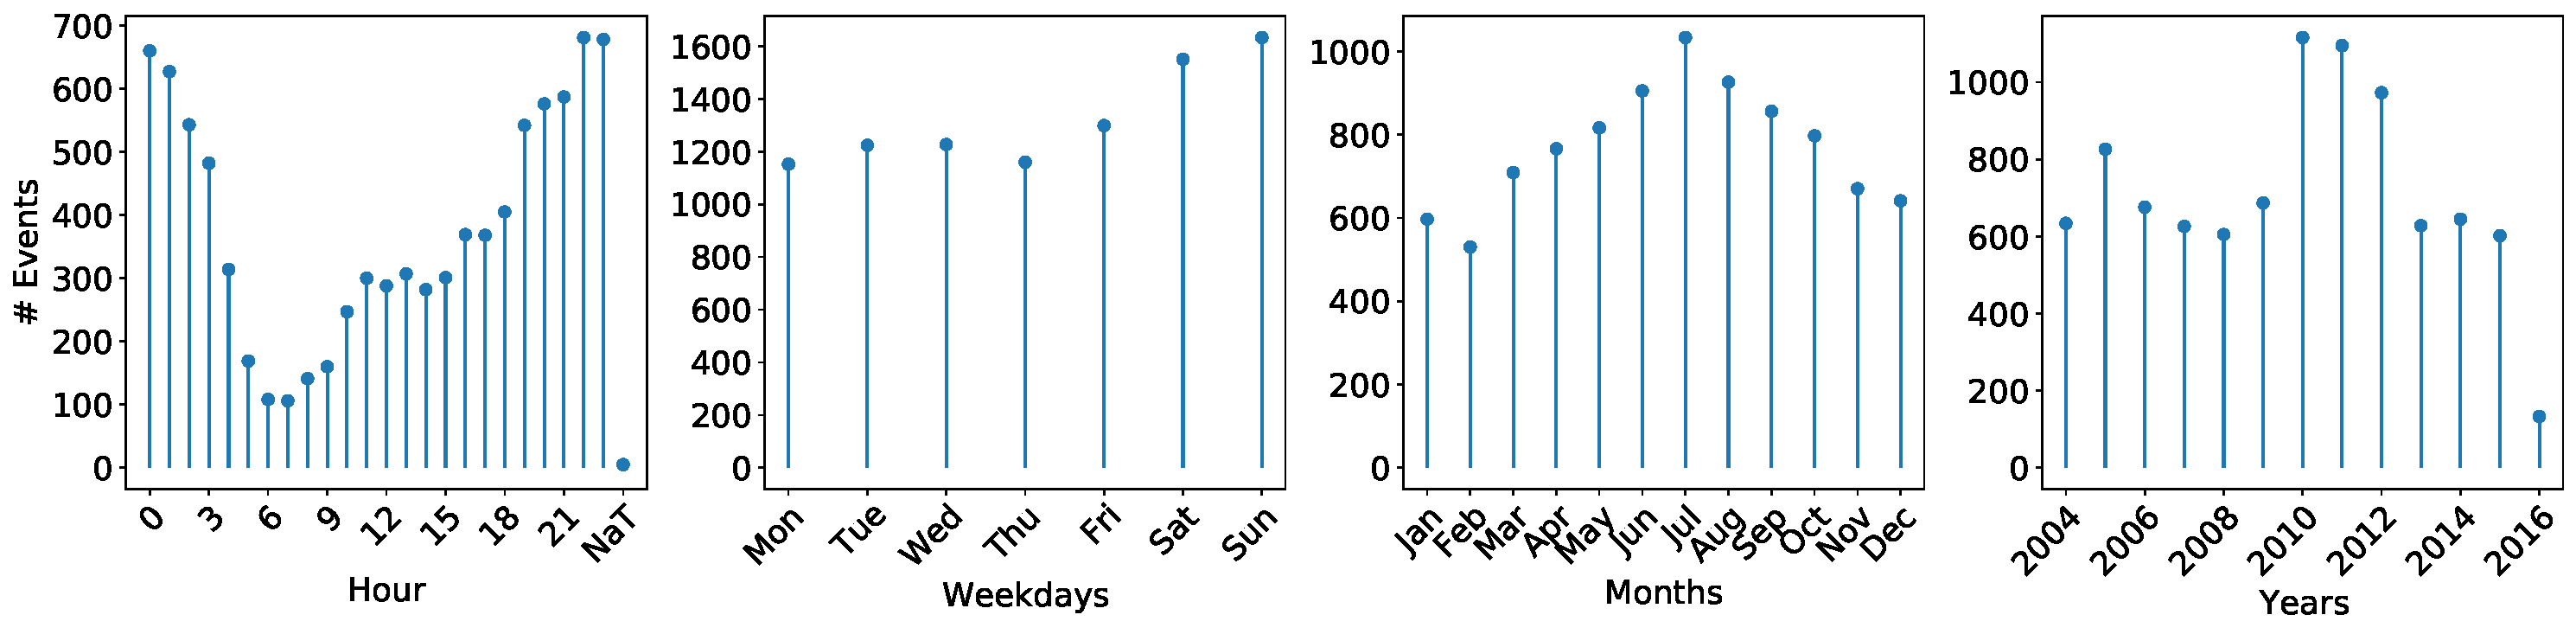
\includegraphics[width=\textwidth]{figs/trrs_times} 
	\caption{Temporal data for TRRs. Left: time during the day; mid-left: time during the week; mid-right: month; right: year.} \label{fig:trrs_times}
\end{figure}

\begin{figure}[h] 
\begin{subfigure}{0.45\textwidth}
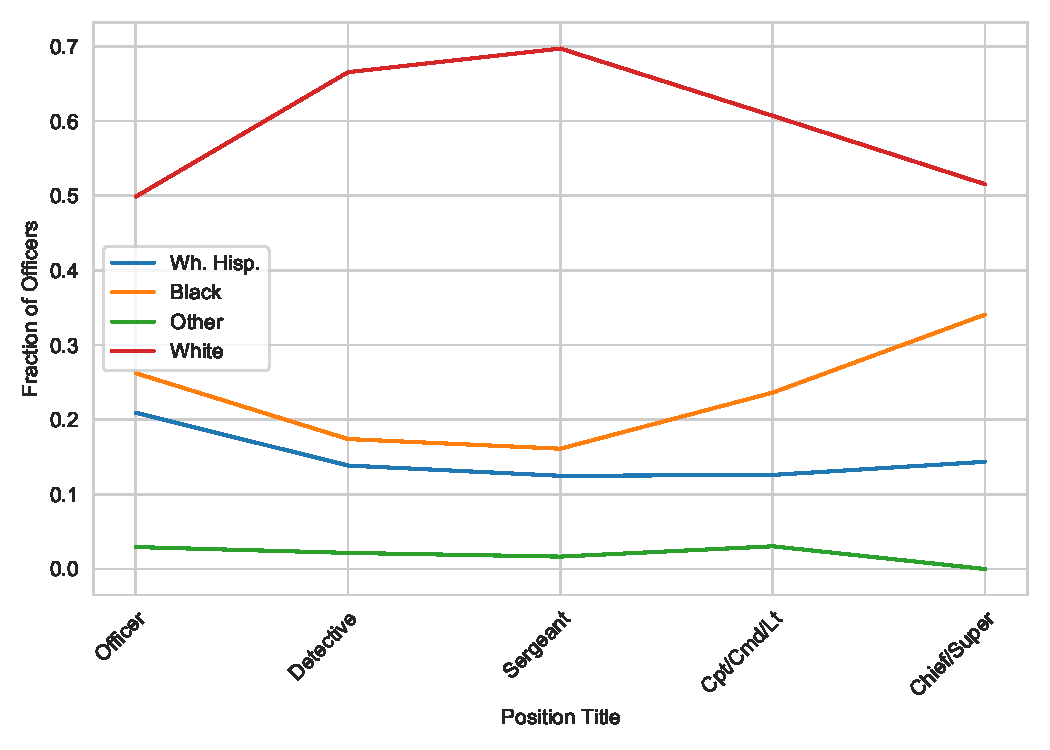
\includegraphics[width=\textwidth]{figs/position_race} 
\end{subfigure}
\begin{subfigure}{0.45\textwidth}
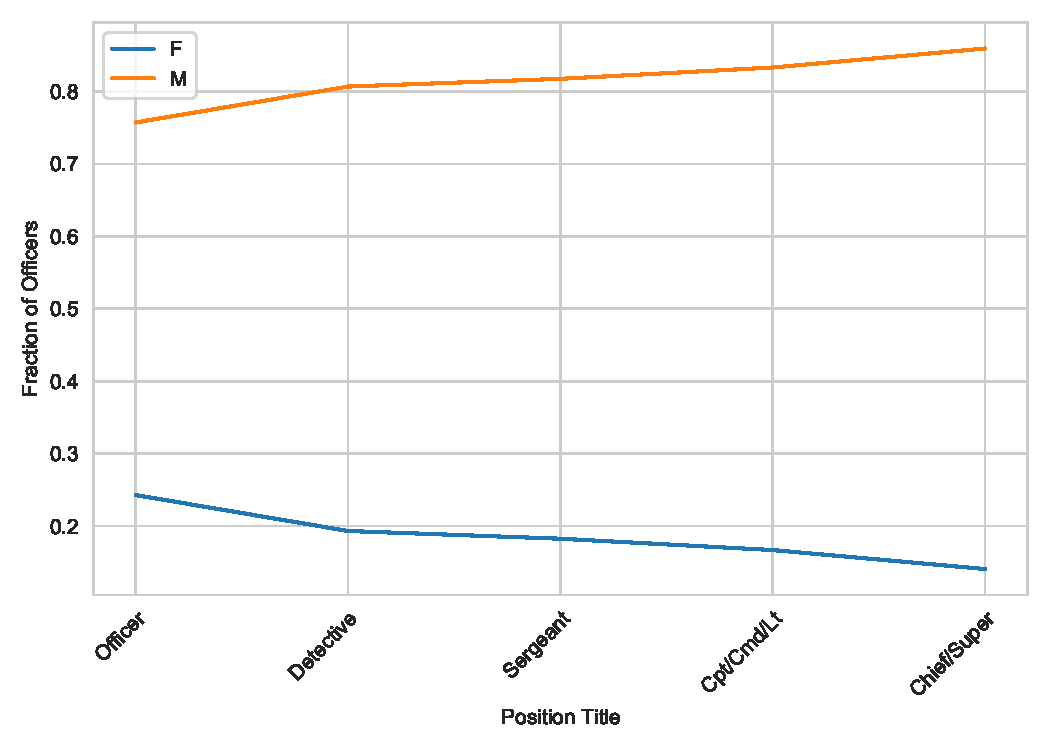
\includegraphics[width=\textwidth]{figs/position_gender} 
\end{subfigure}
\caption{Historical data from the CPD. Fraction of officers in representative positions 
per race category.} \label{fig:position}
\end{figure}



\begin{figure}[h] 
	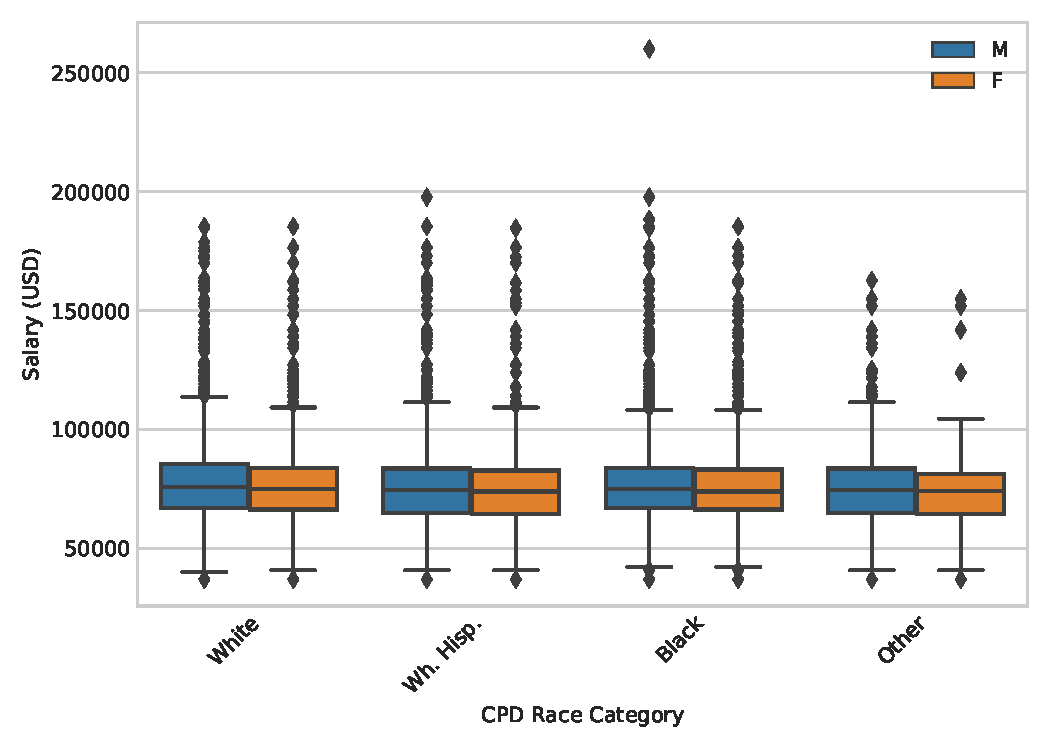
\includegraphics[width=\textwidth]{figs/salary_by_race_gender} 
	\caption{Temporal data for TRRs. Left: time during the day; mid-left: time during the week; mid-right: month; right: year.} \label{fig:salary_gender_race}
\end{figure}

\begin{figure}[h]
	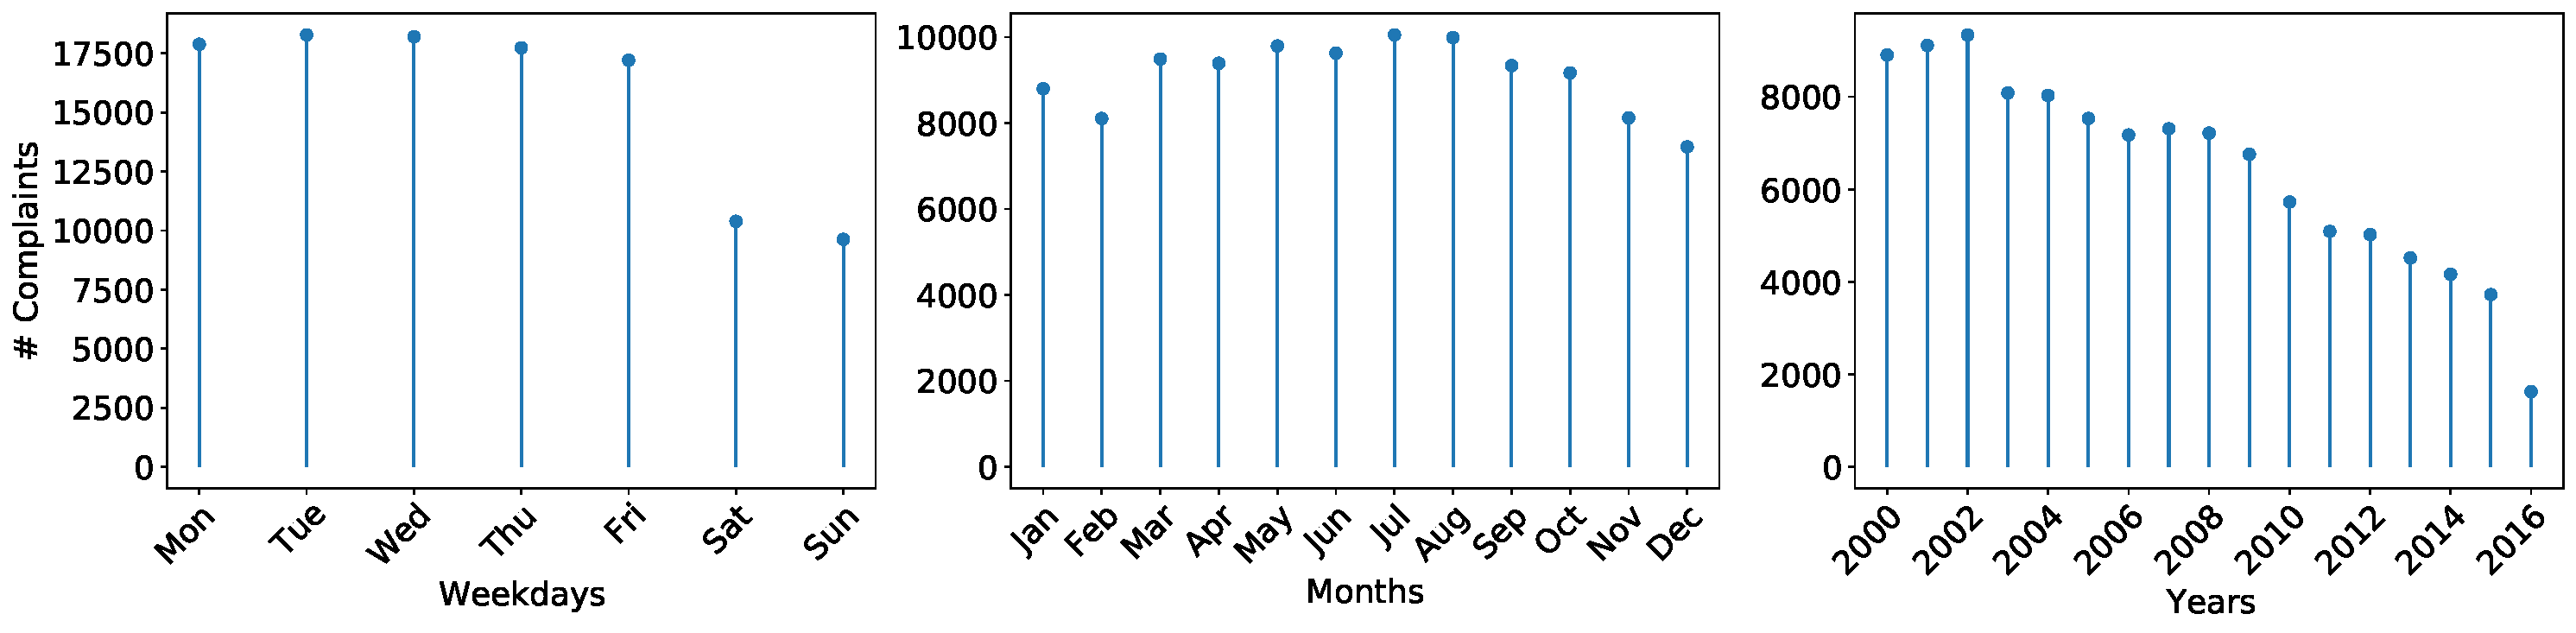
\includegraphics[width=\textwidth, clip, trim= 0 0 460 0]{figs/complaints_times} 
\caption{Complaints per day, month}
\end{figure}





\end{document}
